\documentclass[]{mosi}

% ===== Template packages (kept) =====
%\usepackage{helvet}
\usepackage{amsmath} 
\usepackage{natbib}
\usepackage{graphicx}
\usepackage{subcaption} 

\usepackage[toc,page,header]{appendix}
%\usepackage[utf8]{inputenc} % allow utf-8 input
\usepackage[T1]{fontenc}    % use 8-bit T1 fonts
\usepackage{hyperref}       % hyperlinks
\usepackage{url}            % simple URL typesetting
\usepackage{booktabs}       % professional-quality tables
%\usepackage{lmodern}        % scalable Latin Modern fonts
\usepackage{amsfonts}       % blackboard math symbols
\usepackage{nicefrac}       % compact symbols for 1/2, etc.
\usepackage{microtype}      % microtypography
\usepackage{wrapfig}

\usepackage{amssymb}        % special symbols
% \usepackage{fontawesome}    % icons
\usepackage{titletoc}
\usepackage{minitoc}

\usepackage{array}
\usepackage{etoolbox}
\newcommand{\maxbold}[1]{\textbf{#1}}
\definecolor{lightblue}{RGB}{200, 230, 255}  
\definecolor{headerblue}{RGB}{150, 200, 255} 

\usepackage{pgfplots}
\usepackage{xcolor}
\usepackage{float}
\usepackage{comment}
\usepackage{multirow}
\usepackage{makecell}
\usepackage{siunitx}
\usepackage{tikz}
\usepackage{pgf-pie}
\usepackage[export]{adjustbox}

\usepackage{ragged2e}
\usepackage{tabularx}
\usepackage{caption}
\usepackage{enumitem}
\usepackage{pifont}
\usepackage[hang,flushmargin]{footmisc}

\usepackage{tcolorbox}
\tcbuselibrary{breakable}
\tcbuselibrary{skins}

\usepackage{tabularx}
\usepackage{listings}

\usepackage{inconsolata}

%Including images in your LaTeX document requires adding
%additional package(s)
\usepackage{algorithm}
\usepackage{algorithmic}
\usepackage{adjustbox}
\usepackage{multirow}
\usepackage{tcolorbox}
\usepackage[table]{xcolor}
\usepackage{nicematrix}
\usepackage{booktabs} 
\usepackage{amsmath}
\usepackage{float}
\usepackage{xspace}
\usepackage{subcaption}
\usepackage{calc} % 必须引入,用于计算宽度
\usepackage{cleveref}


% ===== Added to support original content (template-only changes) =====
\usepackage{threeparttable}
\usepackage{setspace}
% \usepackage[a4paper, margin=1in]{geometry}
\usepackage[scheme=plain]{ctex} % needed for Chinese text in appendix prompts

\crefname{figure}{Fig.}{Figs.}
\crefname{table}{Tab.}{Tabs.}
\crefname{section}{Sec.}{Secs.}
\crefname{equation}{Eq.}{Eqs.}
\crefname{appendix}{App.}{Apps.}

% ===== Colors used in original content =====
\definecolor{MossCyan}{HTML}{82D9FF} 
\definecolor{MossBlue}{HTML}{82B1FF}

% ===== Template macros (kept) =====
%\def\axisLabels{{CharXiv, MMBench, MMMU, MMMU-Pro, MathVerse, MathVision, MathVista}}
\def\numAxes{7}
\definecolor{ForestGreen}{RGB}{34, 139, 34}
\definecolor{Red}{RGB}{255, 0, 0}
\newcommand{\catA}{\makecell{3D Spatial \\ Perc. \& Under.}}
\newcommand{\catB}{\makecell{Pattern Recog. \\ \& Matching}}
\newcommand{\catC}{\makecell{Multi-step \\ Reasoning}}
\newcommand{\catD}{\makecell{Strategic \\ Planning}}
\definecolor{tickG}{rgb}{0.1, 0.588, 0.1}
\definecolor{crossR}{rgb}{0.588, 0.1, 0.1}
\newcommand{\cmark}{\textcolor{tickG}{\ding{52}}}
\newcommand{\xmark}{\textcolor{crossR}{\ding{56}}}
\newcommand{\titleLogo}{%
    $\raisebox{-1.5mm}
    {\includegraphics[width=0.05\textwidth]{figures/HERMES_logo.pdf}}$ 
}

\definecolor{frenchblue}{rgb}{0.0, 0.45, 0.73}
\definecolor{babyblue}{rgb}{0.54, 0.81, 0.94}
\definecolor{classicrose}{rgb}{0.98, 0.8, 0.91}
\definecolor{beige}{rgb}{0.96, 0.96, 0.86}
\definecolor{forestgreen}{HTML}{2e7d43}

\definecolor{blue1}{HTML}{91BBE6}
\definecolor{blue2}{HTML}{3F90E0}
\definecolor{blue3}{HTML}{316FAD}

\definecolor{color1}{HTML}{FF9999}
\definecolor{color2}{HTML}{FF6666}
\definecolor{color3}{HTML}{FF3333}
\definecolor{color4}{HTML}{E60000}
\definecolor{color5}{HTML}{B30000}
\definecolor{color6}{HTML}{8CD98C}
\definecolor{color7}{HTML}{53c653}
\definecolor{color8}{HTML}{00B050}
\definecolor{color9}{HTML}{2d862d}
\definecolor{color10}{HTML}{206020}
\definecolor{color11}{HTML}{cca300}
\definecolor{HermesBlue}{RGB}{0,102,204}

\newcommand{\hermes}{\textcolor{HermesBlue}{\textit{\textbf{HERMES}}}\xspace}

% ===== Prompt box from template (kept) =====
\newtcolorbox{promptbox}[2][]{
    colback=white,
    coltext=black,
    arc=3mm,
    boxrule=0.5pt,
    colframe=black!60!white,
    title={#2},
    colbacktitle=black,
    coltitle=white,
    fonttitle=\bfseries,
    top=8pt,
    bottom=8pt,
    left=10pt,
    right=10pt,
    breakable,
    before upper={%
        \linespread{1}\selectfont
        \setlength{\parskip}{1ex plus 0.2ex minus 0.2ex}%
        \setlength{\parindent}{0pt}%
    },
    #1
}

% ===== Title & Author (moved into mosi template) =====
% \title{MOSS Transcribe Diarize: Accurate Transcription with Speaker Diarization}
\title{\titleLogo \hermes: KV Cache as Hierarchical Memory for Efficient Streaming Video Understanding}


\author{
Haowei Zhang$^{1,*}$\hspace{.1em}
Shudong Yang$^{1,2,*}$\hspace{.1em}
Jinlan Fu$^{1,3,\dagger}$ \hspace{.1em}
See-Kiong Ng$^{3}$ \hspace{.1em}
Xipeng Qiu$^{1,2}$ \hspace{.1em}
}
\affiliation{
  $^1$Fudan University, $^2$Shanghai Innovation Institute,
  $^3$National University of Singapore
}
% \affiliation[1]{Fudan University}
% \affiliation[2]{Shanghai Innovation Institute}
% \affiliation[3]{National University of Singapore,}
% \affiliation[4]{OpenMoss Team}


% ===== Abstract (content unchanged) =====
\abstract{
\begin{abstract}
\noindent Recent advancements in Multimodal Large Language Models (MLLMs) have demonstrated significant improvement in offline video understanding. However, extending these capabilities to streaming video inputs, remains challenging, as existing models struggle to simultaneously maintain stable understanding performance, real-time responses, and low GPU memory overhead. To address this challenge, we propose \hermes, a novel training-free architecture for real-time and accurate understanding of video streams. Based on a mechanistic attention investigation, we conceptualize KV cache as a hierarchical memory framework that encapsulates video information across multiple granularities. During inference, \hermes reuses a compact KV cache, enabling efficient streaming understanding under resource constraints. Notably, \hermes requires no auxiliary computations upon the arrival of user queries, thereby guaranteeing real-time responses for continuous video stream interactions, which achieves 10$\times$ faster TTFT compared to prior SOTA. Even when reducing video tokens by up to 68\% compared with uniform sampling, \hermes achieves superior or comparable accuracy across all benchmarks, with up to 11.4\% gains on streaming datasets.
\end{abstract}
}

% ===== Checkdata (mapped from original links) =====
\checkdata[Correspondence]{\email{hwzhang25@m.fudan.edu.cn}, \email{jinlanjonna@gmail.com}}
\checkdata[Homepage]{\url{https://hermes-streaming.github.io/}}
\checkdata[Repository]{\url{https://github.com/haowei-freesky/HERMES}}

% \checkdata[Huggingface Space]{\url{https://huggingface.co/spaces/OpenMOSS-Team/MOSS-transcribe-diarize}}

\newcommand{\todo}[1]{\textcolor{purple}{\bf\small [TODO: #1]}}

\newcommand{\llava}{LLaVA-OV-7B\xspace}
\newcommand{\llavasmall}{LLaVA-OV-0.5B\xspace}
\newcommand{\qwen}{Qwen2.5-VL-7B\xspace}
\newcommand{\qwenbig}{Qwen2.5-VL-32B\xspace}

\definecolor{grey}{RGB}{128,138,135}

\begin{document}
\maketitle
\begingroup
\renewcommand{\thefootnote}{\fnsymbol{footnote}}
\setcounter{footnote}{1}
\footnotetext{Equal contribution.}
\setcounter{footnote}{2}
\footnotetext{Corresponding author.}
\endgroup

% ===== Original meta lines (content unchanged) =====
% \begin{spacing}{1.0}
% {\small \noindent \textbf{Date:} December 31, 2025 \par}
% {\small \noindent \textbf{Demo:} \url{https://openmoss.github.io/MOSS-Transcribe-Diarize-demo/} \par}
% {\small \noindent \textbf{Huggingface Space:} \url{https://huggingface.co/spaces/OpenMOSS-Team/MOSS-transcribe-diarize} \par}
% \end{spacing}

% ===== Original content starts here (sections/tables/figures unchanged) =====

% 为了方便修改,我们可以先定义一个统一的高度变量
\newlength{\myfigheight}
\setlength{\myfigheight}{7.01cm} % 在这里统一调整三张图的高度

\begin{figure*}[t]
    \centering
    
    % --- 子图 (a) ---
    \begin{subfigure}{\widthof{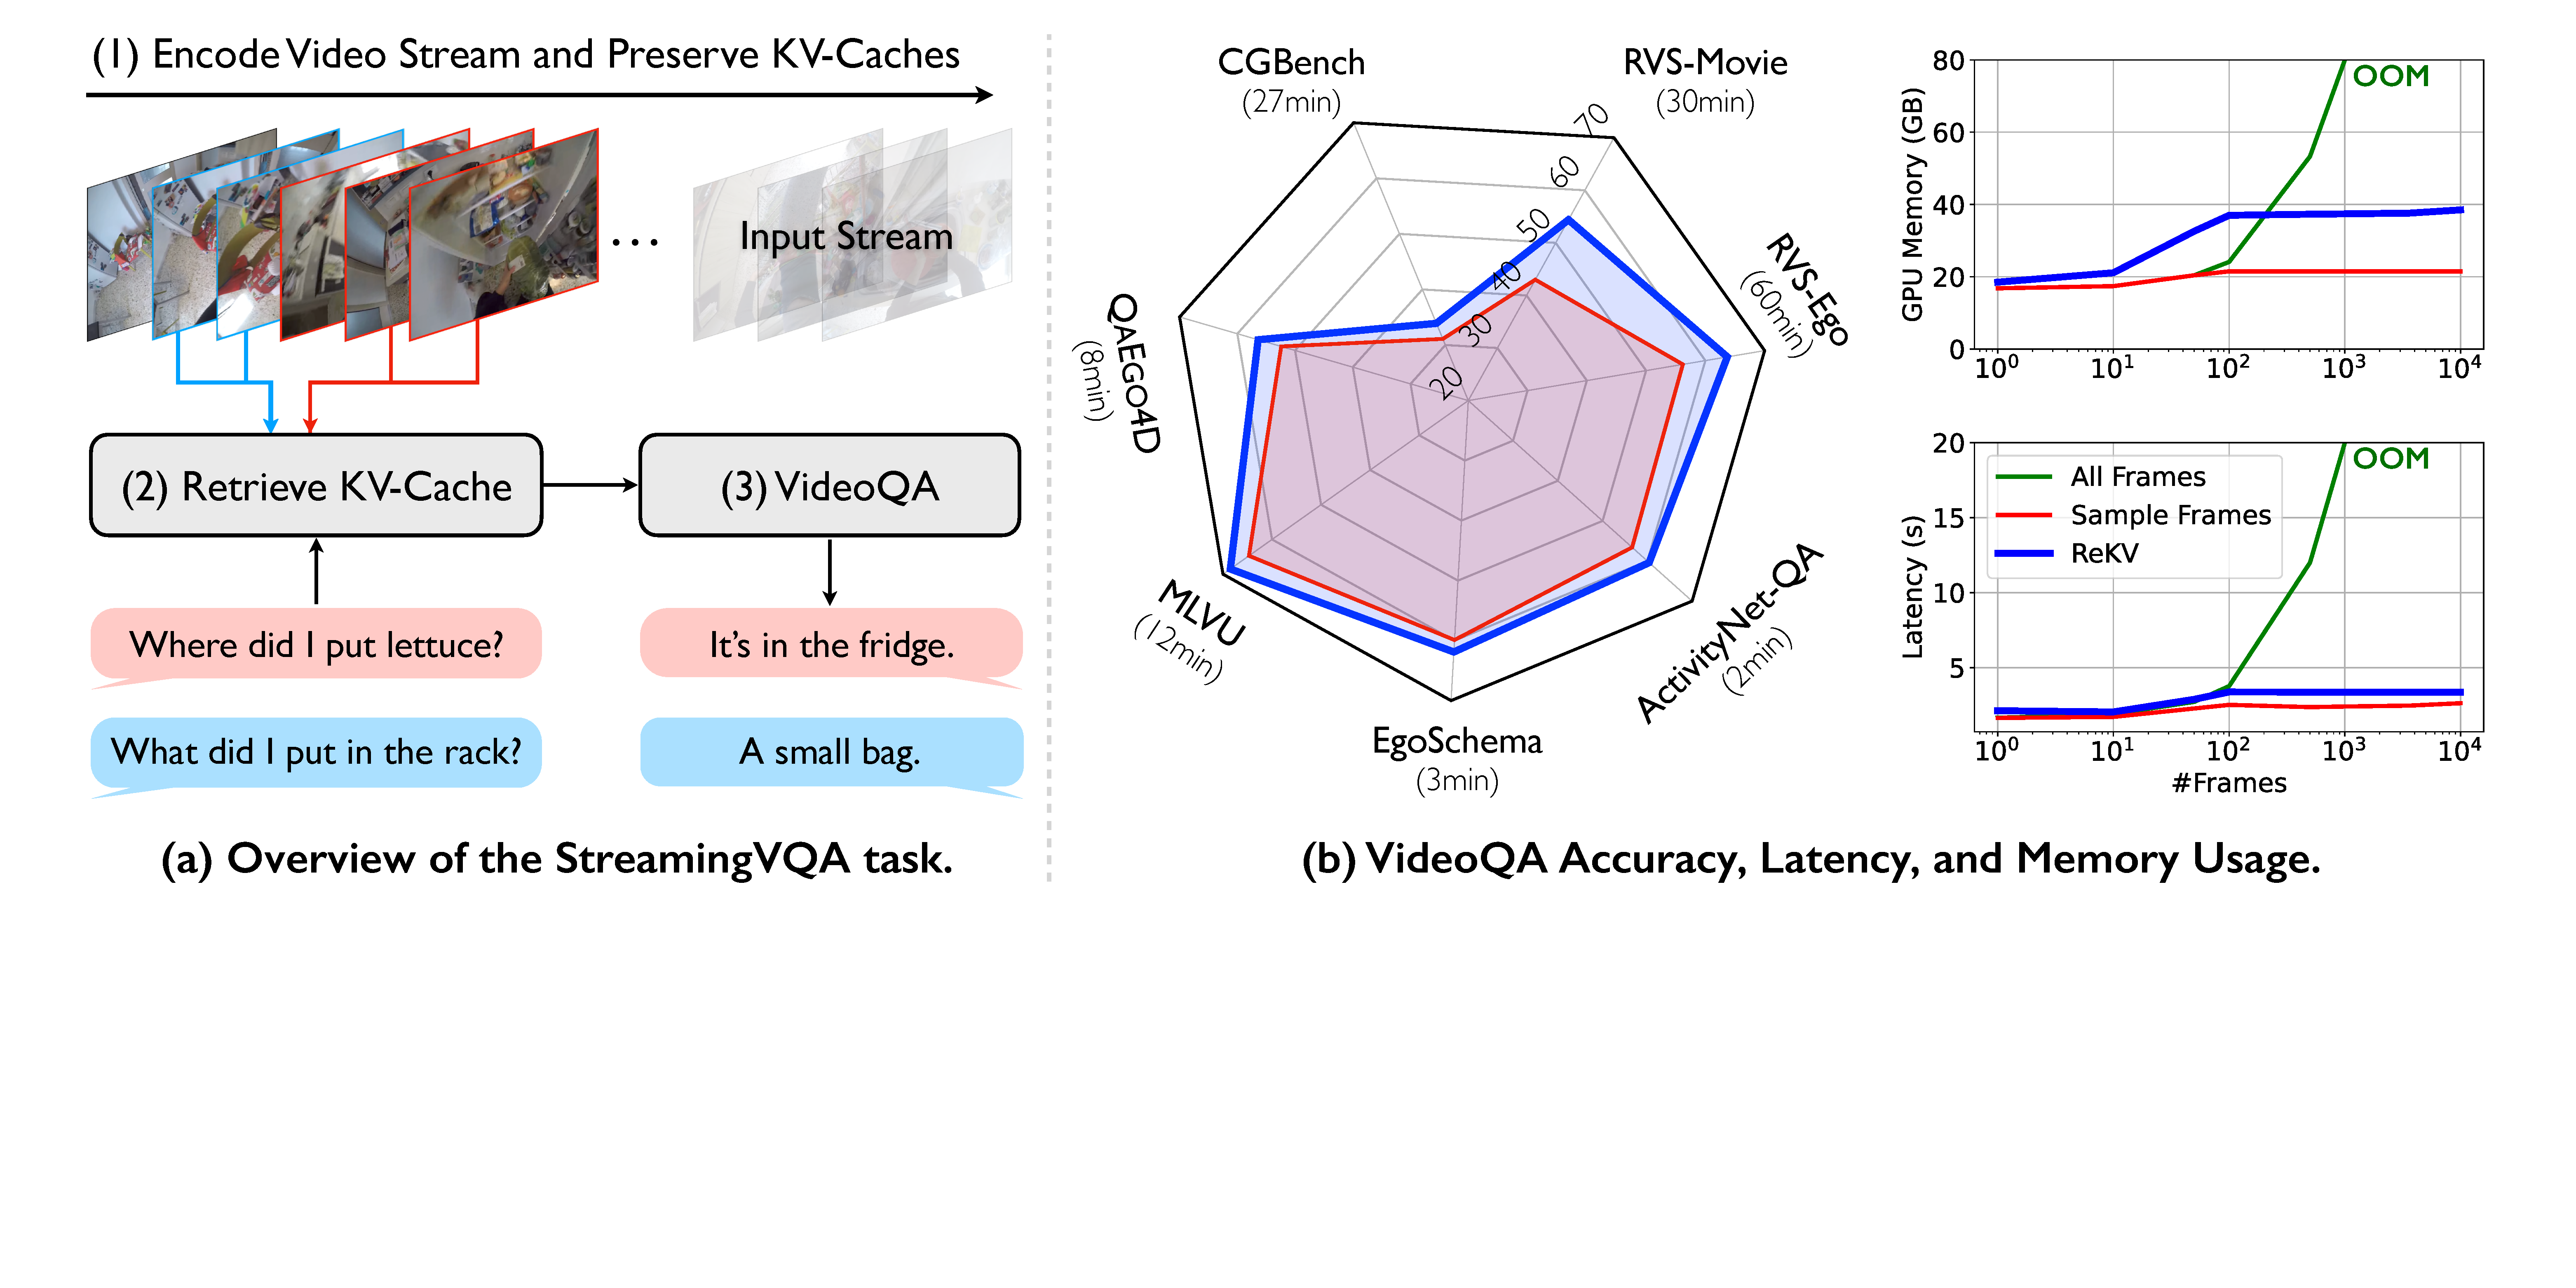
\includegraphics[height=\myfigheight, trim={0 0 415pt 0}, clip]{figures/teaser.pdf}}}
        \centering
        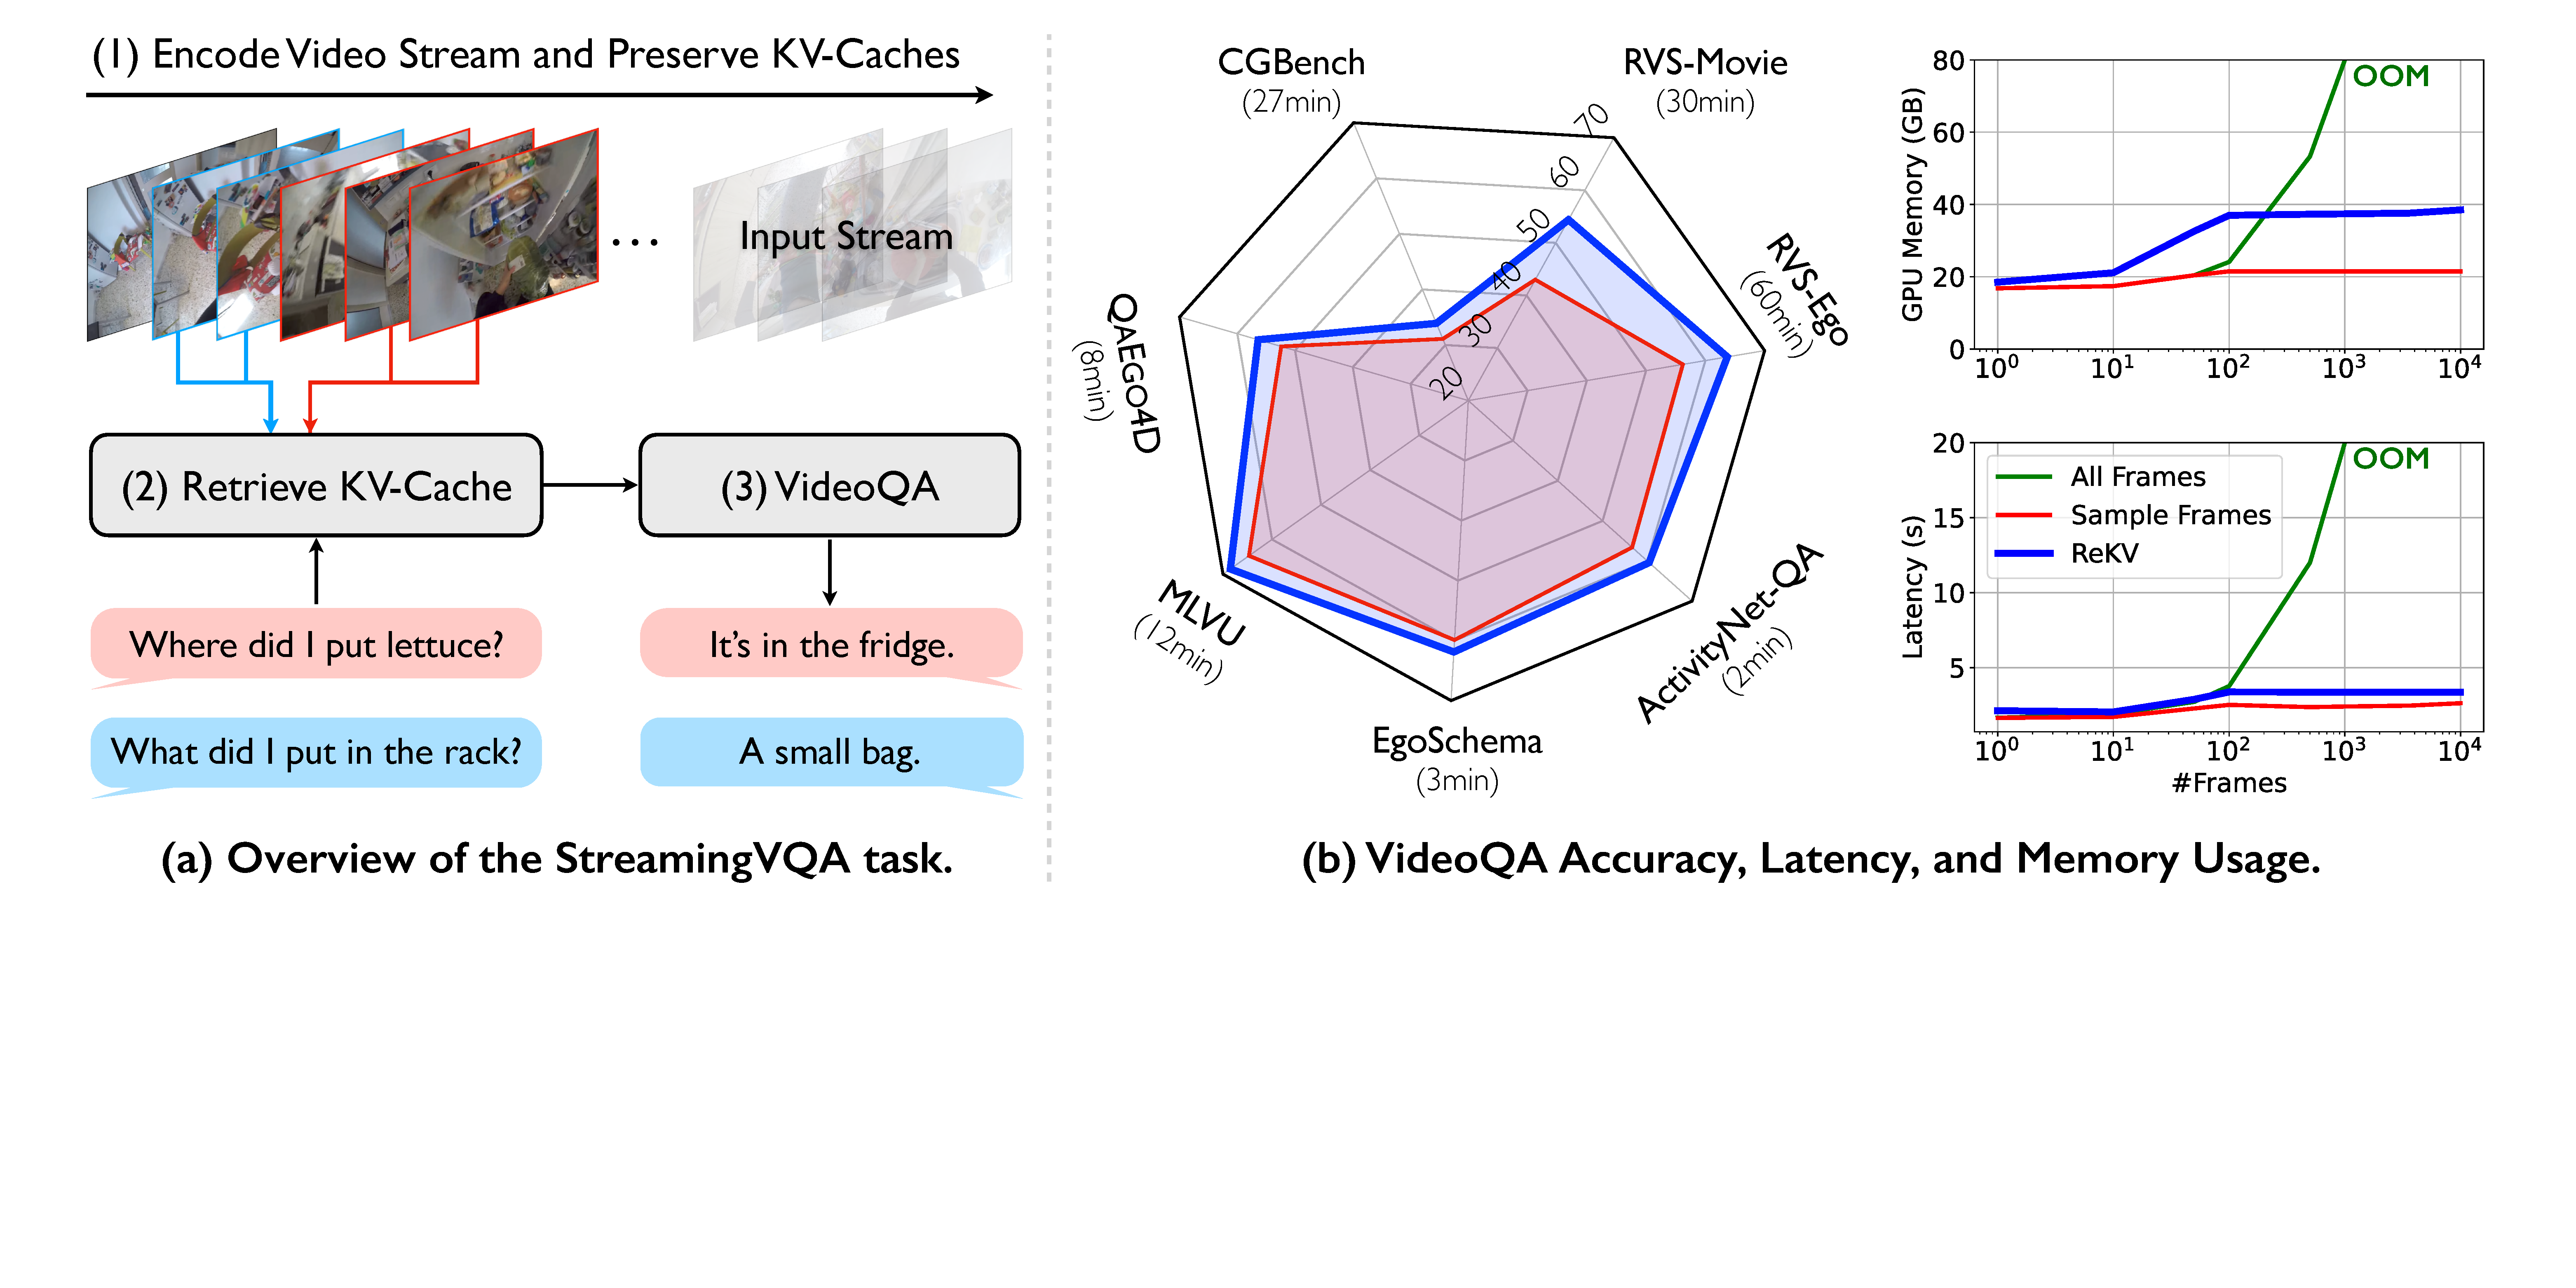
\includegraphics[height=\myfigheight, trim={0 0 415pt 0}, clip]{figures/teaser.pdf}
        \caption{\hermes Framework}
        \label{fig:teaser_a}
    \end{subfigure}
    % --- 子图 (b) ---
    \begin{subfigure}{\widthof{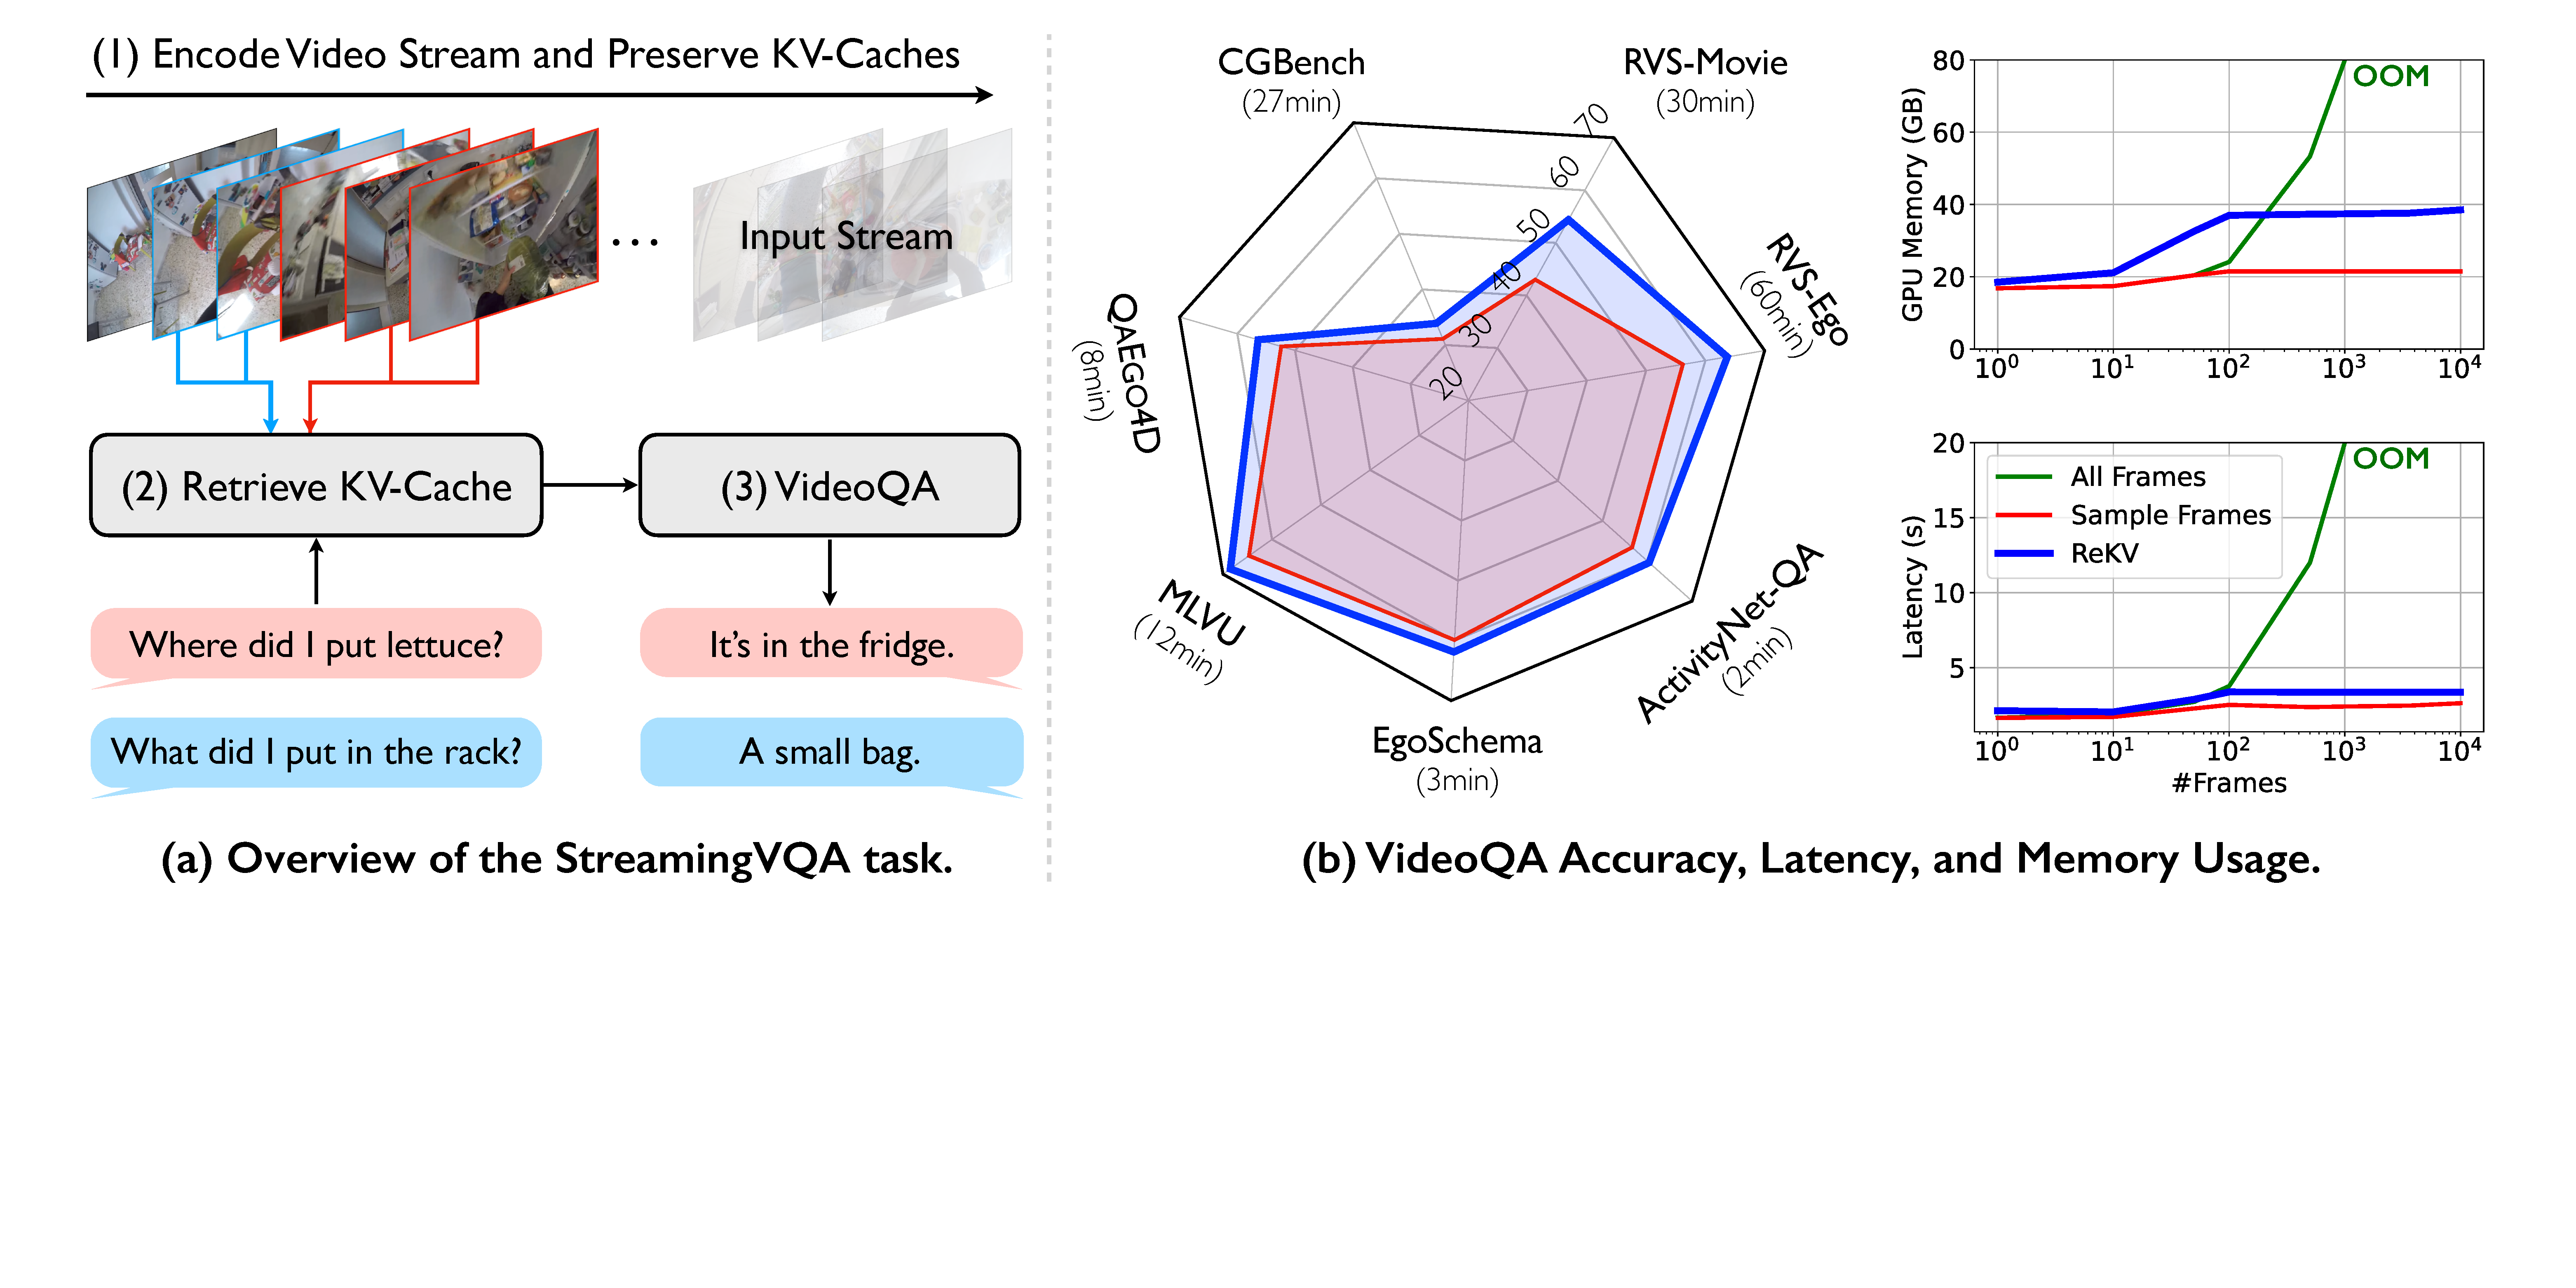
\includegraphics[height=\myfigheight, trim={365pt 0 251pt 0}, clip]{figures/teaser.pdf}}}
        \centering
        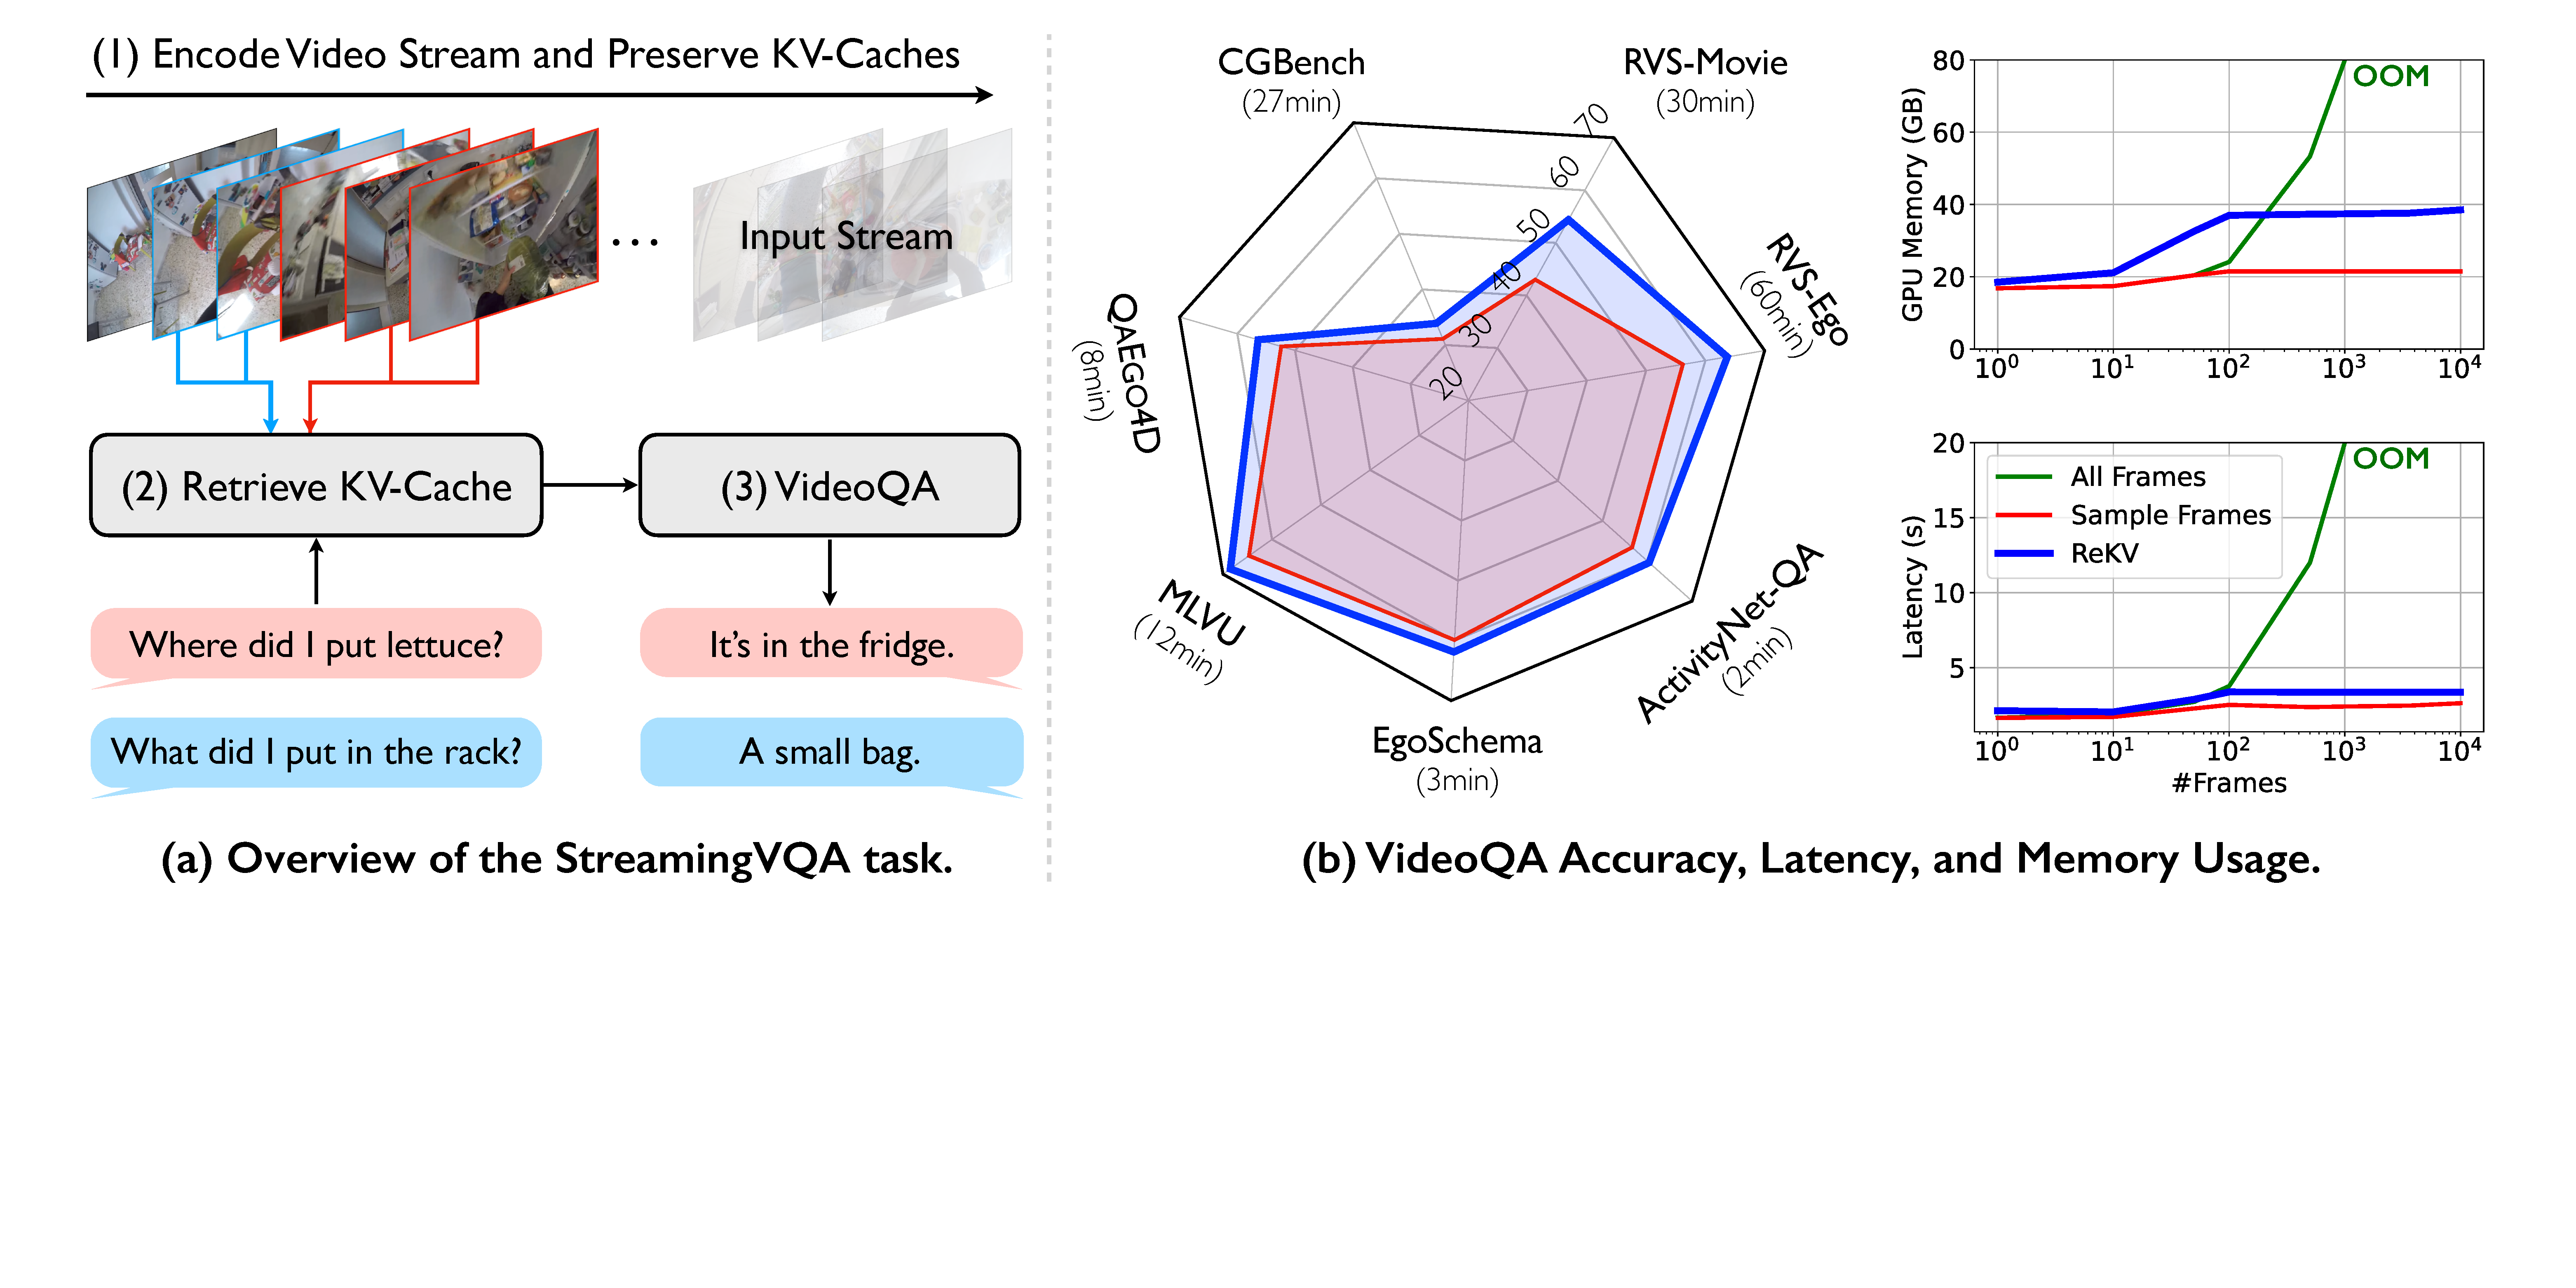
\includegraphics[height=\myfigheight, trim={365pt 0 251pt 0}, clip]{figures/teaser.pdf}
        \caption{Attention Analysis}
        \label{fig:teaser_b}
    \end{subfigure}
    % --- 子图 (c) ---
    \begin{subfigure}{\widthof{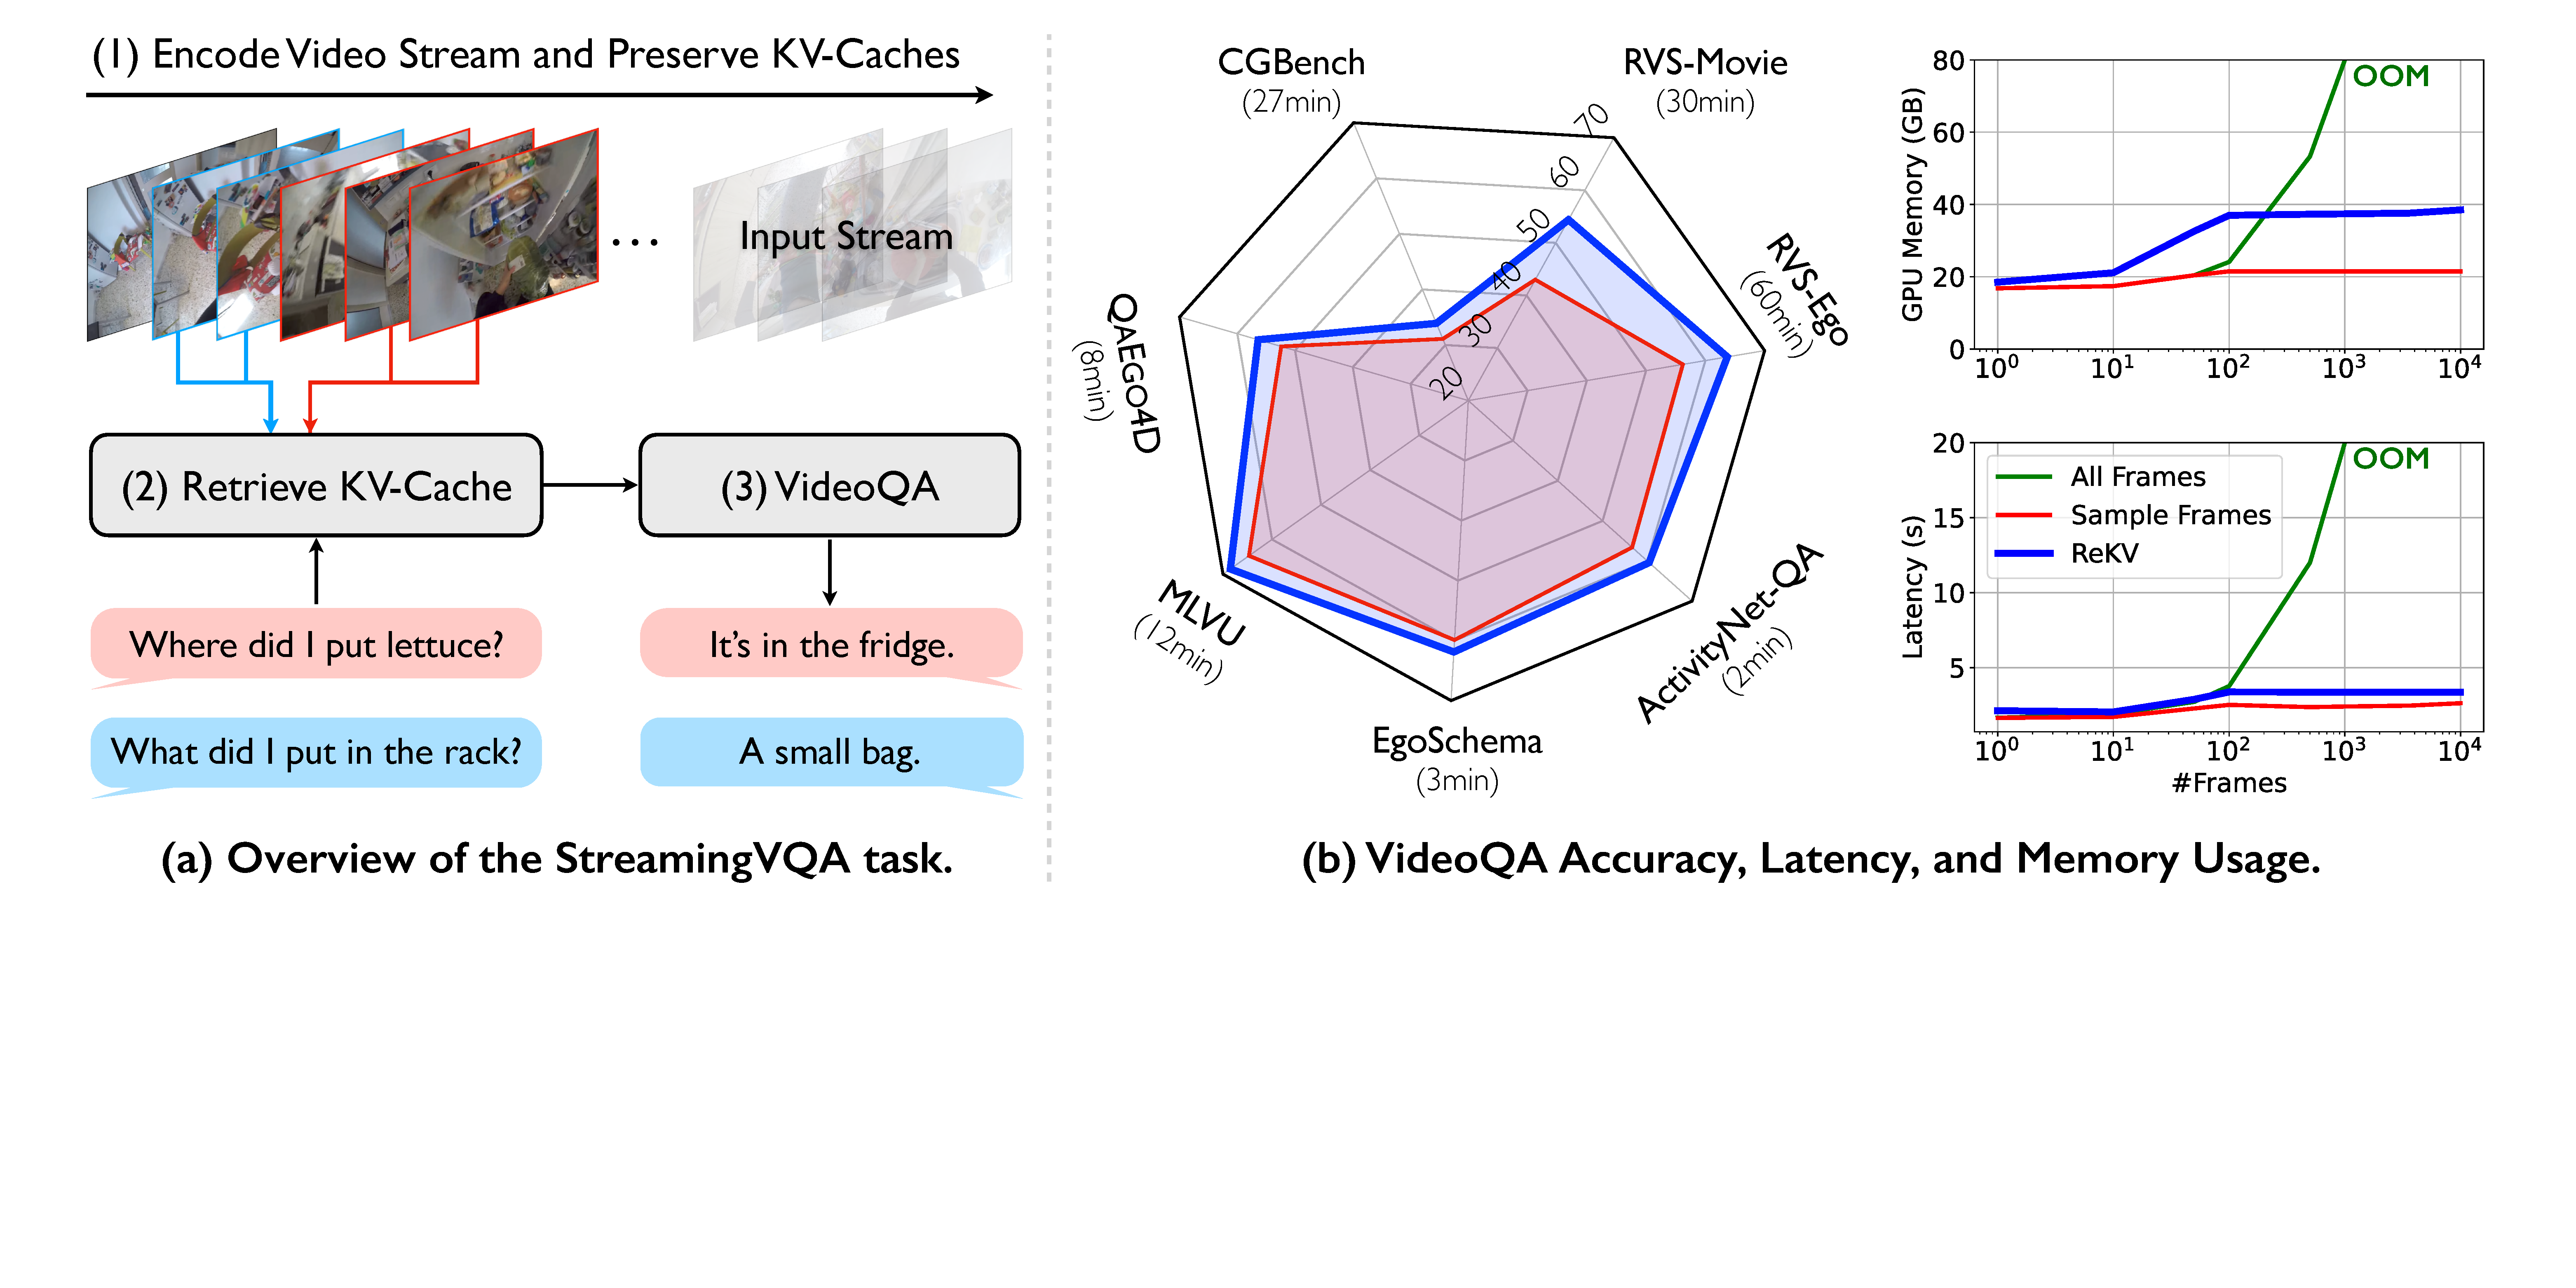
\includegraphics[height=\myfigheight, trim={529pt 0 0 0}, clip]{figures/teaser.pdf}}}
        \centering
        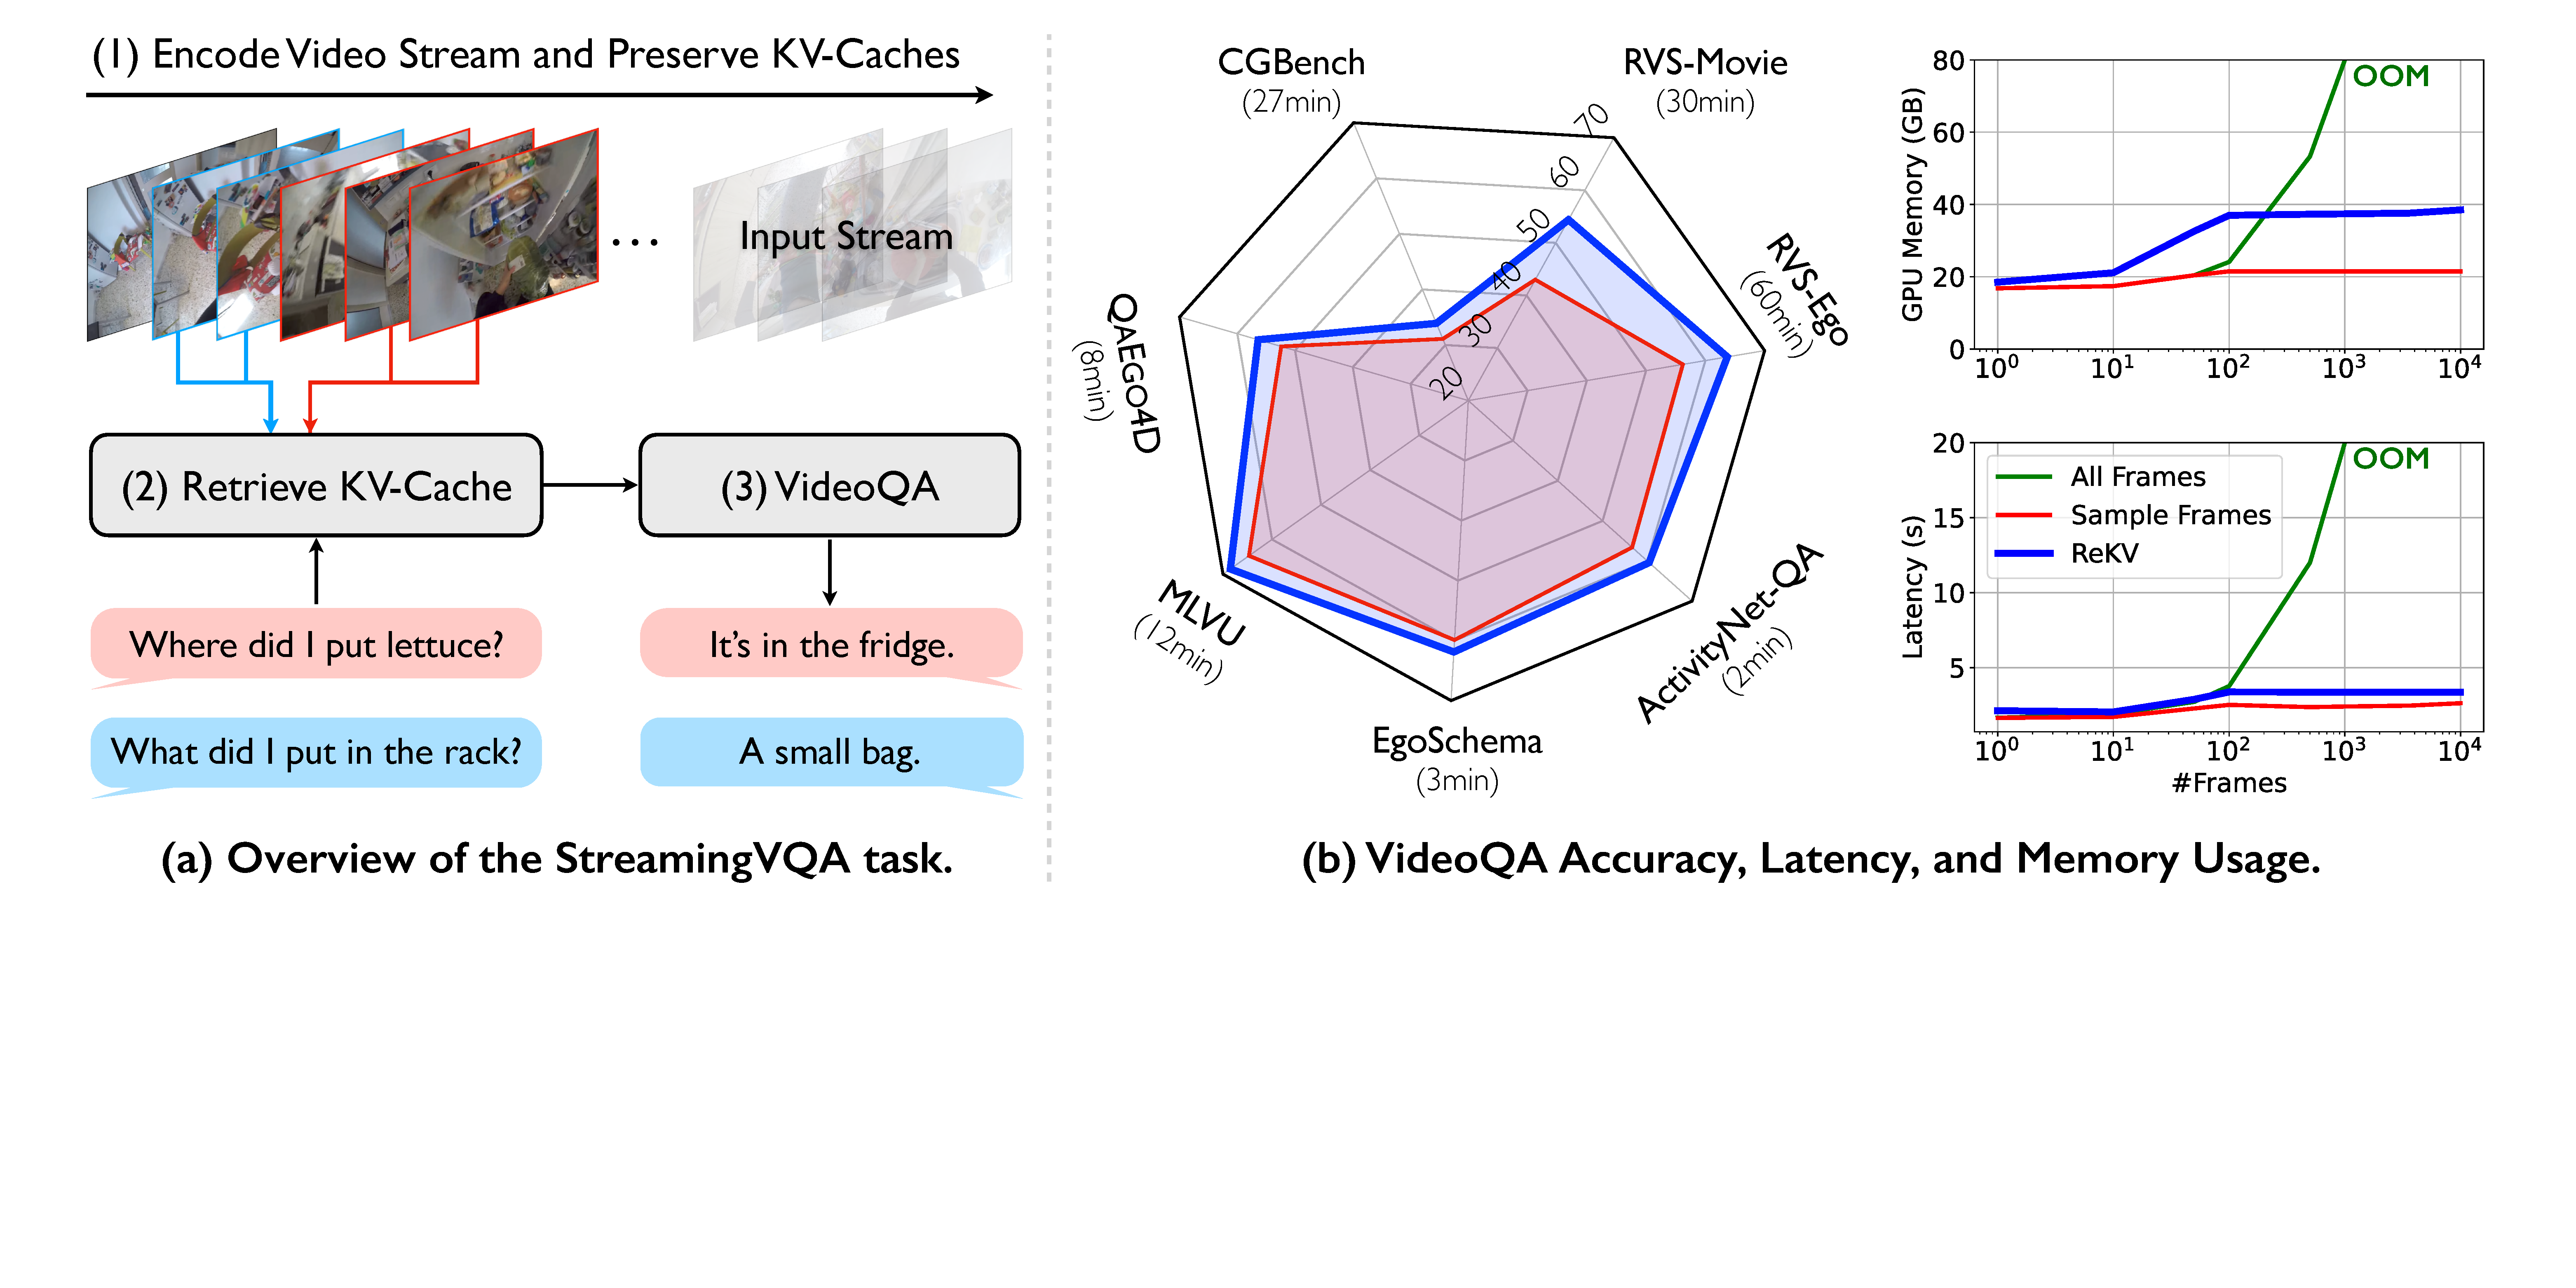
\includegraphics[height=\myfigheight, trim={529pt 0 0 0}, clip]{figures/teaser.pdf}
        \caption{Efficiency Test}
        \label{fig:teaser_c}
    \end{subfigure}
    \caption{\textbf{Left}: \hermes is a training-free approach for efficient streaming video understanding, enabling stable inference by reusing KV cache and performing hierarchical management of video tokens stored in KV cache. \textbf{Middle}: \hermes is based on a mechanistic investigation of the layer-wise attention preferences over hierarchical video information. \textbf{Right}: We evaluate \llava on a single A800 GPU (80 GB). As input frames increase, \hermes consistently maintains extremely low latency (TTFT < 30 ms) and stable GPU memory consumption, exhibiting no risk of OOM errors and requiring no auxiliary external computational resources.}
\end{figure*}



\section{Introduction}
\label{sec:introduction}

% 必须强调流式视频推理的三个重点:1. 稳定准确的推理性能(accuracy) 2. 实时响应 3. 方便端侧设备部署的低GPU memory usage

% 流式输入带来的新挑战

Recent years have witnessed remarkable evolution in the capabilities of Multimodal Large Language Models (MLLMs) in video understanding tasks~\cite{gemini25, li2024llavaonevisioneasyvisualtask, bai2025qwen3vltechnicalreport}.
% Specifically, these models have demonstrated comprehensive understanding and reasoning abilities across various temporal durations and diverse downstream tasks~\cite{li2024mvbenchcomprehensivemultimodalvideo, fu2025videommefirstevercomprehensiveevaluation, mangalam2023egoschemadiagnosticbenchmarklongform}.
Despite the progress, the rapid emergence of real-time applications demands stable long video understanding, low-latency response, and memory-efficient deployment. 
%Consequently, the research frontier is shifting from offline paradigms to streaming video understanding.
%has imposed rigorous demands on MLLMs regarding long temporal context understanding, low-latency inference, and memory efficiency. Consequently, the research frontier is shifting from traditional offline inference paradigms toward streaming inference capable of processing continuous video inputs.
% 现有的offline compression方法由于流式输入的特殊性,无法直接使用
However, existing MLLMs struggle to simultaneously satisfy these requirements on streaming videos.
% Some works streaming methods necessitate expensive model-specific training~\cite{wang2025streambridgeturningofflinevideo, xu2025streamingvlmrealtimeunderstandinginfinite, zeng2025streamforestefficientonlinevideo}, leaving training-free approaches relatively underexplored.
Notably, TimeChat-Online~\cite{timechatonline} observes that a large number of streaming video tokens are redundant, motivating compression methods to address these challenges. While numerous compression techniques have been proposed for offline videos~\cite{wang2025videotreeadaptivetreebasedvideo, yang2024visionziplongerbetternecessary, tao2025dycokedynamiccompressiontokens}, most are ill-suited for memory management in streaming scenarios, as streaming inputs are unpredictable in future frames and queries.
%posing significant challenges for prior static compression methods.
% 现有流式压缩方法的局限,主要有两点: 1. 依赖外挂式记忆和临时检索,时延高。内置式记忆探索得较少,将记忆能力内化入模型很重要 2. 很多是模型特定的训练方法,开销大,不够通用(相对training-free)

To adapt to streaming inputs, recent research introduces specialized memory management techniques, which generally fall into two paradigms: external memory and internal memory. External memory methods store video content as captions or raw vision patches in databases, and perform ad-hoc retrieval and multimodal prefilling at query time~\cite{xiong2025streamingvideounderstandingmultiround, yang2025streamagentanticipatoryagentsstreaming}, suffering from high latency and a lack of end-to-end cohesion. Additionally, many of these methods necessitate costly model-specific training~\cite{wang2025streambridgeturningofflinevideo, xu2025streamingvlmrealtimeunderstandinginfinite, zeng2025streamforestefficientonlinevideo}. In contrast, internalizing memory directly into the key-value cache (KV cache) remains underexplored, yet is crucial for low-latency responses and seamless end-to-end reasoning over stored video contexts. Moreover, KV cache naturally acts as a latent, model-intrinsic memory~\cite{hu2025memoryageaiagents} that frequently interacts with the video stream, making it particularly suitable for training-free memory management. ReKV~\cite{di2025streamingvideoquestionansweringincontext} and LiveVLM~\cite{ning2025livevlmefficientonlinevideo} are representative training-free, cache-based methods for streaming memory management. They store previous video segments in external CPU or disk and need to perform an additional retrieval when a user query arrives, which still rely on external computational resources and leads to significant latency. StreamMem~\cite{yang2025streammemqueryagnostickvcache} leverages chat template tokens to guide compression but lacks fine-grained KV management and mechanistic interpretability.%\jlfu{Discussing how our method differs from other KV-cache–based approaches (e.g., ReKV, StreamMem, and LiveVLM)}

% 正式介绍HERMES这个方法,顺带再提一个之前工作的不足:缺乏机制可解释性

To overcome the aforementioned limitations of existing streaming video methods, we propose \hermes (KV Cache as \underline{\textbf{H}}i\underline{\textbf{ER}}archical \underline{\textbf{M}}emory for \underline{\textbf{E}}fficient \underline{\textbf{S}}treaming Video Understanding), a training-free and plug-and-play approach that can be seamlessly integrated into existing MLLMs. %as shown in \cref{fig:teaser}. 
Grounded in a mechanistic investigation of layer-wise attention shown in~\cref{fig:teaser_b}, we conceptualize KV cache as a hierarchical memory framework that stores video information across multiple levels of granularity: 
%shallow layers as sensory memory, deep layers as long-term memory and middle layers as transitional working memory.
shallow layers function as sensory memory, exhibiting a strong recency bias toward newly arriving frames; deep layers act as long-term memory, focusing on frame-level rhythmic anchor tokens; and middle layers serve as transitional working memory that balances recency information with frame-level semantic representations.
Our method \hermes comprises three components: \emph{hierarchical KV cache management}, \emph{cross-layer memory smoothing}, and \emph{position re-indexing}. During inference, \hermes reuses the compact KV cache and requires no auxiliary computations or external devices upon the arrival of user queries, thereby guaranteeing real-time responses. Experiments show that \hermes maintains stable and accurate performance with up to 68\% fewer video tokens, while maintaining consistently low response latency and a constant GPU memory footprint.

% In contrast to many prior multimodal compression works that rely on heuristic techniques~\cite{kim2025infinipotvmemoryconstrainedkvcache, yang2025streammemqueryagnostickvcache, chen2025streamkvstreamingvideoquestionanswering}, which struggle with limited interpretability and reliability, our approach is based on a mechanistic investigation of layer-wise attention preference for hierarchical video information.

%Grounded in a mechanistic investigation of layer-wise attention preferences for hierarchical video tokens, we conceptualize the key-value cache (KV cache) as a hierarchical memory framework that stores video information across multiple levels of temporal granularity.

% We observe that the shallow, middle, and deep decoder layers of MLLMs correspond to the short-term, mid-term, and long-term memory of streaming video information, respectively.


% \begin{itemize} [leftmargin=*]
% \itemsep0em 
% \item 
% \textbf{Shallow Layers as Short-term Memory}: For the short-term video memory stored in the shallow layers, where attention exhibits a strong preference for temporally recent video tokens, we employ a First-In-First-Out (FIFO) eviction strategy to only keep the recent video tokens.
% \item
% \textbf{Middle Layers as Mid-term Memory}: The middle layers serve as a transition from short-term to long-term memory. These layers increasingly focus on video content that is temporally distant from the time point of user queries, with attention patterns becoming progressively sparser. Token eviction in this stage is determined by a weighted combination of attention and recency scores of video tokens. To account for unpredictable user queries, we utilize specifically designed local and global guidance prompts to steer the compression.
% \item
% \textbf{Deep Layers as Long-term Memory}: In the deep layers, attention is extremely sparse, and the bias toward recent video tokens largely disappears. These layers primarily capture global and abstract semantic information. Compression is guided by attention scores from the global guidance prompt. To maximize the preservation of video information, evicted tokens are aggregated into a summary token maintained at the end of the sequence.
% \end{itemize}

%Beyond the hierarchical design, we introduce \emph{layer consistency} as a smoothing mechanism. This allows the long-term memory in deeper layers to provide feedback for token retention in earlier layers, thereby mitigating information inconsistencies across different memory stages. 

% Finally, to support potentially infinite video streams, especially in resource-limited scenarios, we maintain a fixed and compact GPU memory footprint at all times. We implement a \emph{soft position encoding reassignment} method to ensure both stable comprehension performance and an enhanced perception of recent temporal dynamics, which are essential for streaming understanding~\cite{xu2025streamingvlmrealtimeunderstandinginfinite}.


To summarize, our main contributions are as follows:
\begin{enumerate}[leftmargin=*]
\itemsep0em 
\item
Grounded in a mechanistic analysis on attention visualization, we pioneer the conceptualization of KV cache as a hierarchical video memory framework across multiple granularities.

\item
We propose \hermes, a training-free method for streaming video understanding by reusing hierarchically managed KV cache. Despite reducing video tokens by up to 68\%, \hermes achieves competitive accuracy, with gains of up to 11.4\% on streaming benchmarks.

\item
\hermes exhibits outstanding efficiency in streaming scenarios. Compared to the prior training-free SOTA method, it achieves up to a 10$\times$ speedup in latency. With a constant, compact GPU memory footprint and no auxiliary computation at query time, \hermes ensures consistently low-latency responses.

\end{enumerate}
\begin{figure*}[!t]
  \centering

  % ---------- 第一行:a 和 c ----------
  % \begin{subfigure}[t]{0.496\textwidth}
  %   \centering
  %   \includegraphics[width=\linewidth]{figures/vis/shallow.pdf}
  %   \caption{Visualization of shallow layer attention.}
  %   \label{fig:shallow_vis}
  % \end{subfigure}
  % \begin{subfigure}[t]{0.496\textwidth}
  %   \centering
  %   \includegraphics[width=\linewidth]{figures/vis/deep.pdf}
  %   \caption{Visualization of deep layer attention.}
  %   \label{fig:deep_vis}
  % \end{subfigure}

\begin{subfigure}[t]{0.246\textwidth}
    \centering
    \includegraphics[width=\linewidth]{figures/vis/layer_00_attention.pdf}
    \caption{Shallow layer attention.}
    \label{fig:shallow_vis}
  \end{subfigure}
  \begin{subfigure}[t]{0.50\textwidth}
    \centering
    \includegraphics[width=\linewidth]{figures/vis/deep.pdf}
    \caption{Deep layer attention.}
    \label{fig:deep_vis}
  \end{subfigure}
  \begin{subfigure}[t]{0.242\textwidth}
    \centering
    \includegraphics[width=\linewidth]{figures/vis/layer_08_attention.pdf}
    \caption{Middle layer attention.}
    \label{fig:mid_vis}
  \end{subfigure}
  

  %\vspace{0em} % ↓ 比 1em 紧很多

  % ---------- 第二行:b ----------
  % \begin{subfigure}[t]{\textwidth}
  %   \centering
  %   \includegraphics[width=\linewidth]{figures/vis/mid_horizon.pdf}
  %   \caption{Visualization of middle layer attention.}
  %   \label{fig:mid_vis}
  % \end{subfigure}
  \caption{Visualization of the average attention weights (log scale) for user queries over video tokens in \llava with a FIFO KV cache budget of 6K video tokens per layer, averaged across 300 user video questions.}
  \label{fig:layer_vis}
\end{figure*}

% \begin{figure*}[!t]
%   \centering

%   % ---------- 第一行:a 和 c ----------
%   \begin{subfigure}[t]{0.496\textwidth}
%     \centering
%     \includegraphics[width=\linewidth]{figures/vis/shallow.pdf}
%     \caption{Visualization of shallow layer attention.}
%     \label{fig:shallow_vis}
%   \end{subfigure}
%   \begin{subfigure}[t]{0.496\textwidth}
%     \centering
%     \includegraphics[width=\linewidth]{figures/vis/deep.pdf}
%     \caption{Visualization of deep layer attention.}
%     \label{fig:deep_vis}
%   \end{subfigure}

%   %\vspace{0em} % ↓ 比 1em 紧很多

%   \caption{Visualization of the average attention weights over video tokens in \llava under a sliding window size of 6,000 video tokens, averaged across 300 user video questions.}
%   \label{fig:layer_vis}
% \end{figure*}
% \todo{Fig2: delete one line as the placeholder}



%\section{Mechanistic Investigation: Layer-wise Preference for Hierarchical Video Information}
\section{Layer-wise Preference for Hierarchical Streaming Video Information}
\label{sec: investigation}

% In this section, we perform a mechanistic investigation of attention preferences in MLLM decoder layers, uncovering how different layers specialize in storing multiple-granularity video memory.

Sliding Window is a standard paradigm for streaming video processing by incrementally encoding the continuous video stream chunk by chunk. When KV cache reaches the pre-defined memory budget, token eviction is triggered, and deciding which tokens to keep is crucial for stable understanding. Existing methods~\cite{di2025streamingvideoquestionansweringincontext, yang2025streammemqueryagnostickvcache, xu2025streamingvlmrealtimeunderstandinginfinite} rely on coarse-grained eviction strategies such as FIFO uniformly across all layers, overlooking layer-wise attention preferences.

To fill this gap, we conduct a mechanistic investigation of attention preferences in MLLM decoder layers, revealing how layers specialize in storing multiple-granularity video memory. To derive generalized insights, we randomly sample 100 video-question pairs from each of the short (62s\footnote{To ensure the sliding window contains 6,000 tokens, a video at 0.5 fps for LLaVA-OV must have a duration of at least $6,000 / 196 / 0.5\approx 62s$.} - 141s), medium (251s - 1,092s) and long (1,795s - 3,579s) duration subsets of the VideoMME benchmark~\cite{fu2025videommefirstevercomprehensiveevaluation} to cover diverse video durations and user queries. The video samples are uniformly sampled at 0.5 fps and subsequently fed into \llava in a streaming chunk-wise manner, with each chunk containing 8 frames. \llava consists of 28 decoder layers, and each video frame is uniformly encoded into 196 visual tokens. During the prefilling stage for video tokens, we maintain a constant budget $|M|$ of 6K video tokens per KV cache layer. After each eviction step, the positional indices of tokens per KV cache layer are re-indexing to contiguous [0, $|M|$).

Layer-wise attention visualizations over video tokens maintained in a FIFO KV cache in~\cref{fig:layer_vis} reveal three general stages of attention preference, along with more visualization results presented in~\cref{app:attn_vis}:

\begin{itemize} [leftmargin=*]
\itemsep0em
\item
\textbf{Shallow Layers as Sensory Memory}:
As shown in~\cref{fig:shallow_vis}, the shallow layers (e.g., layer 0) exhibit an intense recency bias, with attention sharply concentrated on the most recent visual tokens and rapidly decaying over earlier ones. This behavior aligns with the concept of \emph{Sensory Memory}~\cite{ATKINSON196889, shan2025cognitivememorylargelanguage}: shallow layers function as a short-lived buffer for the most recent visual inputs, enabling the model to quickly perceive incoming frames.

\item 
\textbf{Deep Layers as Long-term Memory}: % or semantic Memory
In deep layers (e.g., layer 26 in~\cref{fig:deep_vis}), recency bias largely disappears. Instead, the attention pattern becomes highly sparse and rhythmic, with local extrema appearing at regular intervals. These extrema are exactly N = 196 tokens apart, matching to the number of tokens encoding a single frame in \llava. These local maxima can be regarded as frame-level "anchor tokens", summarizing the visual information of each frame. This pattern reflects \emph{Long-term Memory}~\cite{ATKINSON196889, shan2025cognitivememorylargelanguage}: deep layers store critical frame-level semantic representations for long-horizon understanding.

\item 
\textbf{Middle Layers as Working Memory}:
Middle layers (e.g., layer 8 in~\cref{fig:mid_vis}) exhibit a gradual reduction in recency bias, with attention more evenly distributed across recent and earlier tokens. Simultaneously, the attention begins to transition toward the rhythmic patterns in the deep layers. This behavior corresponds to \emph{Working Memory}~\cite{BADDELEY197447, hu2025memoryageaiagents}: middle layers integrate recent and earlier visual information, bridging short-term sensory traces with frame-level semantic summaries.
% Therefore, the middle layers serve as a transitional memory stage, bridging the short-term, recency-focused attention of shallow layers with the long-range, frame-level semantic attention of deep layers.
%This layer-wise investigation of attention preferences over video tokens provides a solid interpretability foundation for the concrete hierarchical KV cache management strategies.

\end{itemize}



\section{StreamingVQA: Task Definition and Discussion} 
\label{sec:task}

This paper considers the problem of streaming video question-answering (\textbf{StreamingVQA}), where a model continuously processes a video stream and can respond to questions about past visual content at any moment. 
In this section, we formally define the task and outline the design principles for our proposed solution.

Given a video stream $\mathcal{V}^T := [v_1, v_2, ..., v_T]$ consisting of $T$ frames and a set of $N$ questions $\mathcal{Q} := \{q_1, q_2, \dots, q_N\}$,
StreamingVQA aims to answer a question $q_i$ at any time step $t~(1 \le t \le T)$, using only the frames seen up to that point, $\mathcal{V}^t := [v_1, v_2, ..., v_t]$.


\noindent\textbf{Discussion-I: StreamingVQA {\em vs.}~OfflineVQA.} StreamingVQA involves continuously analyzing an incoming video stream and answering questions based on the observed visual content at any moment. 
In contrast, conventional video question-answering models~\citep{frozen_bilm,video_chatgpt,llava_next_video,llava_onevision} operate in an offline mode, referred to as OfflineVQA.
The two paradigms differ in that: 
1) StreamingVQA processes a continuous video stream, while OfflineVQA handles a predefined video input, and 
2) StreamingVQA allows questions to be asked at any point during the stream, whereas OfflineVQA processes questions only after the entire video has been viewed.
Notably, OfflineVQA can be considered a special case of StreamingVQA, where all questions are posed after the video is fully processed. 


Conventional approaches typically employ a visual encoder~\citep{clip,siglip,fang2023eva} and a projection module~\citep{llava_next_video,blip2} to process video frames~($\mathcal{V}^t$).
The output is concatenated with the tokenized question to form a sequence $[\mathcal{V}_t, q_i]$~\footnote{We maintain the original notation for simplicity.}, which is then passed to an LLMs to predict an answer.
However, this approach is impractical due to the high computational cost associated with processing a large number of frames ($T$).


A common workaround is sparse frame sampling~\citep{video_chatgpt, llava_next_video, llava_onevision}, 
but this introduces new problems:
(i) loss of critical visual information, leading to incomplete or inaccurate responses, and
(ii) the need to reprocess frames for different questions, since questions asked at different time points require distinct frame samples. This becomes increasingly inefficient as $T$ and $N$ grow.

Given these challenges, current OfflineVQA methods fall short when applied to StreamingVQA scenarios. Therefore, designing a new approach optimized for StreamingVQA is crucial to handling video streams more efficiently, enabling real-time question answering and unlocking more interactive video analysis applications.


\noindent\textbf{Discussion-II: Design Principles for Efficient StreamingVQA.} 
To tackle the aforementioned challenges, we can exploit the causal nature of the LLM decoder to avoid redundant computations and strike a balance between accuracy and speed. 
During attention calculations, causal masking prevents the model from accessing future tokens, ensuring that video tokens are encoded independently of the questions. This allows us to \textit{decouple video encoding from question-answering}.

For video encoding, we leverage the KV-Cache optimization to accelerate inference.
However, as number of frames grows large, handling the massive number of video tokens becomes increasingly inefficient and may exceed the model’s capacity~\citep{lm_infinite,streamingllm}.
To address this, we adopt a sliding-window attention mechanism~\citep{lm_infinite}, which limits the attention scope to only the most recent frames.

Regarding question-answering, Video KV-Caches are stored and can be reused as context to answer different questions. 
However, long video sequences produce a substantial amount of KV-Caches, leading to excessive GPU memory consumption, computational overhead, and unnecessary distractions if all are used.
To address this, we introduce an efficient retrieval method that selects the most relevant video key-value vectors from the video KV-Caches. These selected vectors then serve as context, enabling efficient and scalable StreamingVQA.




\section{
\ourmethod: \underline{Re}trieve In-context Video \underline{KV}-Cache
}
\label{sec:method}

This section introduces \textbf{\ourmethod}, an approach that integrates seamlessly with a Video-LLM to enable efficient StreamingVQA without requiring additional training.
Overall, \ourmethod~efficiently encodes the video stream, maintains its KV-Caches, retrieves relevant caches based on the given question, and uses them for accurate question-answering.

\begin{figure}[t]
\centerline{\includegraphics[width=.85\linewidth]{figures/src/framework.pdf}}
\caption{
\textbf{Overview of~\ourmethod.}
We modify the attention mechanism in Decoder-based Video-LLMs:
(a) The video stream is encoded with sliding-window attention (Equation~\ref{equ:video_encoding}), with out-of-window Video KV-Caches offloaded to RAM or disk.
(b) Upon receiving a question, relevant key-value vectors are retrieved based on cosine similarity, with compressed vectors to accelerate retrieval (Equation~\ref{equ:retrieval}).
(c) The retrieved key-value vectors are reloaded onto the GPU and utilized for autoregressive answer generation (Equation~\ref{equ:answer_generation}).
}
\label{fig:framework} 
\end{figure}

We aim to enable Video-LLMs, trained on limited frames, 
to perform StreamingVQA \textbf{without additional training}.
As shown in Figure~\ref{fig:framework}, 
the proposed \ourmethod~has three components: 
video stream encoding, video KV-Cache retrieval, and question-answering using the retrieved key-value vectors.

\noindent\textbf{Video Stream Encoding with Sliding-window Attention.} 
We encode the video stream $\mathcal{V}^T$ incrementally, processing it chunk by chunk.
At each step, the inputs include past key-value vectors $\mathbf{P} = \{(\mathbf{k}_j, \mathbf{v}_j)\}_{j=1}^{l_P}$ and the current tokens $\mathbf{X}=\{\mathbf{t}_{i+l_P}\}_{i=1}^{l_X}$, 
where $l_P$ denotes the lengths of past key-values, and $l_X$ refers to the chunk size.
The local key-value vectors within a window $l_L$ can thus be derived as 
$\mathbf{L} = \mathbf{P}_{[l_P - l_L + 1 : l_P]}$.
The attention calculation is then formulated as:
\begin{equation}
    \mathbf{O} = \text{Attn}\left(\mathbf{W_Q}\mathbf{X}, [\mathbf{L}_k, \mathbf{W_K}\mathbf{X}], [\mathbf{L}_v, \mathbf{W_V}\mathbf{X}]\right),
    \label{equ:video_encoding}
\end{equation}
where $\mathbf{W_Q}$, $\mathbf{W_K}$, and $\mathbf{W_V}$ are the attention layer parameters, $\mathbf{L}_k$ and $\mathbf{L}_v$ correspond to the key and value vectors in $\mathbf{L}$. All video KV-Caches are stored for future retrieval. For extremely long videos, we manage memory constraints by offloading KV-Caches to RAM or disk, as in~\citep{infllm}.

\noindent\textbf{External Video KV-Cache Retrieval.} 
Here, we utilize an external CLIP-like model~\citep{clip, siglip} to retrieve question-relevant video KV-Cache, primarily as a baseline to assess whether retrieval can enhance VideoQA performance, as demonstrated in Section~\ref{sec:experiments}. 
Specifically, a CLIP-like model transformers each video frame into a vector $\mathbf{v} = f_v(v) \in \mathrm{R}^D$, where $f_v$ represents the visual encoder, $D$ denotes the vector dimension. Similarly, the question is encoded as $\mathbf{q} = f_t(q) \in \mathrm{R}^D$, where $f_t$ is the text encoder. We then compute the cosine similarity between the embeddings of frame and question: 
\begin{equation}
    \text{Sim}(\mathbf{v}, \mathbf{q}) = \frac{\mathbf{v} \cdot \mathbf{q}}{\tau~||\mathbf{v}||~||\mathbf{q}||}
    \label{equ:retrieval}
\end{equation} 
where $\tau$ is a learnable temperature parameter. This similarity is calculated at the frame level, rather than at the token level. Alternatively, we can group $b$ consecutive frames into blocks by averaging their frame vectors and then compute block-level similarity scores. Finally, the $r$ most relevant video frames or $\lceil r/b \rceil$ video blocks are retrieved. The corresponding video KV-Cache, denoted as $\mathbf{R}$, is subsequently loaded onto the GPU for question-answering.

\noindent\textbf{Internal Video KV-Cache Retrieval.} Building on recent advancements in handling long sequences with LLMs~\citep{infllm, quickllama, em_llm}, we further explore using self-attention layers within Video-LLMs for retrieval. Similar to external retrieval, internal retrieval is still performed at the level of video frames or blocks.

During video modeling, the average of the key vectors of a frame is computed as its representative frame vector: $\mathbf{v} = \frac{1}{N_f} \sum_{j=1}^{N_f} \mathbf{k}_j \in \mathrm{R}^{D'}$, where $N_f$ is the number of tokens per frame, and $\mathbf{k}_j$ is the $j$-th key vector. 
To reduce computational overhead, we do not differentiate between attention heads and instead concatenate them into a single vector, with $D'$ as the resultant dimension. Similarly, the question vector is computed as $\mathbf{q} = \frac{1}{N_q} \sum_{k=1}^{N_q} \mathbf{q}_{k} \in \mathrm{R}^{D'}$, where $N_q$ is the number of tokens in the question, 
and $\mathbf{q}_{k}$ is its $k$-th query vector. The similarity computation and video KV-Cache retrieval are identical to that of external retrieval, except that $\tau$ is set to 1.

Note that, internal retrieval offers several advantages over external retrieval. 
First, it operates independently within each self-attention layer, allowing different layers to retrieve different video blocks.\footnote{For simplicity, we omit the layer index in the above explanation.}
This allows for a broader capture of video context. 
Additionally, internal retrieval reuses already computed hidden representations and does not introduce extra parameters, which reduces the computational overhead compared to external retrieval.

\noindent\textbf{Question-Answering Using Retrieved KV.} The retrieved Video KV-Caches serve as the context for video question-answering. Formally, the attention calculation is formulated as:
\begin{equation}
    \mathbf{O} = \text{Attn}\left(\mathbf{W_Q}\mathbf{X}, [\mathbf{R}_k, \mathbf{W_K}\mathbf{X}], [\mathbf{R}_v, \mathbf{W_V}\mathbf{X}]\right),
    \label{equ:answer_generation}
\end{equation} 
where $\mathbf{X}$ represents either the question tokens or the current token being decoded, and $\mathbf{R}_k$ and $\mathbf{R}_v$ are the key and value vectors from the context, which includes the retrieved video, question, and previously generated tokens. 

\noindent\textbf{Positional Encoding.}
Our baseline Video-LLMs employ Rotary Position Embeddings (RoPE)~\citep{su2024roformer}, a commonly used relative positional encoding method.
Our video streaming encoding process follows LM-Infinite~\citep{lm_infinite}, where RoPE operates normally within the local window but is constrained by a ``distance ceiling'' for more distant tokens. 
For question-answering, we do not account for the original positions of the retrieved KV-Caches, as handling unseen distances among tokens presents significant challenges~\citep{lm_infinite}.
Instead, we treat these retrieved tokens as regular consecutive tokens. 
We also experimented with a static variation from Inf-LLM~\citep{infllm}, where all retrieved tokens are assigned the same position. 
Our results show that applying standard RoPE to retrieved video tokens leads to better performance, likely due to the importance of capturing temporal information in video comprehension.

\section{Experiments}
\label{sec:experiments}

\subsection{Experimental Setup}
\paragraph{Benchmarks.}
We evaluate \hermes on diverse streaming and offline benchmarks. For streaming understanding, we use StreamingBench~\cite{lin2024streamingbenchassessinggapmllms}, OVO-Bench~\cite{li2025ovobenchfarvideollmsrealworld} and RVS (including RVS-Ego and EVS-Movie)~\cite{zhang2024flashvstreammemorybasedrealtimeunderstanding}.
%These benchmarks follow the streaming video QA paradigm, limiting the available visual context to only the video content before the current timestamp. Additionally, unpredictable user questions occur at any time.
For offline video evaluation, we adopt one short video dataset MVBench~\cite{li2024mvbenchcomprehensivemultimodalvideo}, along with two long video datasets, VideoMME~\cite{fu2025videommefirstevercomprehensiveevaluation} and Egoschema~\cite{mangalam2023egoschemadiagnosticbenchmarklongform}. We conduct evaluation on the official dev split of Egoschema and report VideoMME results without subtitles. Our benchmark selection covers both multiple-choice and open-ended questions as QA form. The details of utilized benchmarks are demonstrated in~\cref{app:details_of_benchmarks}.

\paragraph{Models.}
To further verify the broad applicability of our method, we select two popular open-source MLLM series, LLaVA-OneVision (LLaVA-OV)~\cite{li2024llavaonevisioneasyvisualtask} and Qwen2.5-VL~\cite{bai2025qwen25vltechnicalreport}. Each is tested across two different parameter scales, covering a large range from 0.5B to 32B. For Qwen2.5-VL, we maintain its native dynamic resolution on video input, ensuring a fair comparison with the base model.

\paragraph{Implementation Details.}
For evaluating \hermes across all benchmarks, each video is encoded and processed chunk by chunk, with 16 frames per chunk, and sequentially prefilling the backbone LLM. Then, token compression is triggered once the predefined memory budget is exceeded.

For the layer partition, we follow the mechanistic investigations presented in ~\cref{sec: investigation}: 10\% shallow, 60\% middle and 30\% deep layers. A more comprehensive analysis of attention behaviors as supportive evidence can be found in~\cref{fig:more_vis}. The cross-layer memory smoothing hyperparameter $\lambda$ proposed in~\cref{sec: smoothing} is layer-dependent, with detailed configurations reported in~\cref{app:smooth_config}.


All evaluations are conducted using FP16 mixed precision and efficiency tests are conducted on a single A800 GPU, consistent with prior works~\cite{di2025streamingvideoquestionansweringincontext, chen2025streamingtomstreamingtokencompression}. Greedy decoding is used to generate deterministic outputs. Accuracy evaluations can be completed on one H200 GPU.

\subsection{Main Results}
\paragraph{Streaming Video Understanding}
\begin{table*}[ht]
\renewcommand{\arraystretch}{0.9}
% \renewcommand\tabcolsep{4.3pt}
    \centering
    \footnotesize
    % 6 columns: Model, Frames, StreamingBench, OVO-Bench-rt, OVO-Bench-backward, OVO-Bench-Avg.
    % \resizebox{0.98\linewidth}{!}{
    \begin{tabular}{l c | c c c c}
    \toprule
    \multirow{2}{*}{\textbf{Model}} & \multirow{2}{*}{\textbf{\#Frames}} & \textbf{StreamingBench} & \multicolumn{3}{c}{\textbf{OVO-Bench}} \\
    & & Real-Time & Real-Time & Backward & \textbf{Avg.} \\
    \midrule
    \midrule
    Human & - & 91.46 & 93.20 & 92.33 & 92.83 \\
    \midrule
    \multicolumn{6}{c}{\textbf{Proprietary MLLMs}} \\
    \midrule
    Gemini 1.5 pro~\cite{gemini25} & 1 fps & 75.69 & 69.32 & 62.54 & 66.41\\
    GPT-4o~\cite{openai2024gpt4ocard} & 64 & 73.28 & 64.46 & 60.75 & 62.87\\
    Claude 3.5 Sonnet~\cite{claude3_5} & 20 & 72.44 & - & - & -\\
    \midrule
    \multicolumn{6}{c}{\textbf{Open-source Offline MLLMs}} \\
    \midrule
    Video-LLaMA2-7B~\cite{videollama2} & 32 & 49.52 & - & - & -\\
    VILA-1.5-8B~\cite{vila} & 14 & 52.32 & - & - & -\\
    Video-CCAM-14B~\cite{videoccam} & 96 & 53.96 & - & - & -\\
    LongVA-7B~\cite{longva} & 128 & 59.96 & - & - & -\\
    Qwen2-VL-7B~\cite{wang2024qwen2vlenhancingvisionlanguagemodels} & 64 & 69.04 & 60.65 & 48.58 & 54.62 \\
    InternVL-V2-8B~\cite{internvl2} & 16 & 63.72 & 60.73 & 44.00 & 52.37 \\
    % Kangaroo-7B~\cite{kangaroo} & 64 & 64.60 & - & - & -\\
    LLaVA-NeXT-Video-32B~\cite{llava-next} & 64 & 66.96 & - & - & -\\
    MiniCPM-V-2.6-8B~\cite{minicpm} & 32 & 67.44 & - & - & -\\
    \addlinespace[1pt]
    
    \midrule
    \multicolumn{6}{c}{\textbf{Open-source  Online MLLMs}} \\
    \midrule
    Flash-VStream-7B~\cite{flashvstream} & - & 23.23 & 29.86 & 25.35 & 27.61\\
    VideoLLM-online-8B~\cite{videollmonline} & 2 fps & 35.99 & 20.79 & 17.73 & 19.26\\
    Dispider-7B~\cite{dispider} & 1 fps & 67.63 & 54.55 & 36.06 & 45.31\\
    TimeChat-Online-7B~\cite{timechatonline} & 1 fps & 75.36 & 61.90 & 41.70 & 51.80\\
    StreamForest-7B~\cite{zeng2025streamforestefficientonlinevideo} & 1 fps & 77.26 & 61.20 & 52.02 & 56.61 \\

    \midrule
    \multicolumn{6}{c}{\textbf{Training-free Offline-to-Online Methods}} \\
    \midrule
    LLaVA-OV-7B~\cite{li2024llavaonevisioneasyvisualtask} & 64 & 71.34 & 63.06 & 43.64 & 53.35 \\

    \hspace{3pt} + ReKV~\cite{di2025streamingvideoquestionansweringincontext} & 0.5 fps &  69.22 & 57.33 & 44.16 & 50.75 \\

    \hspace{3pt} + LiveVLM~\cite{ning2025livevlmefficientonlinevideo} & 0.5 fps & 72.92 & - & - & -\\

    \hspace{3pt} + StreamKV~\cite{chen2025streamkvstreamingvideoquestionanswering} & 0.5 fps & 68.80 & - & - & -\\

    \rowcolor{gray!20}  \hspace{3pt} + HERMES (6K tokens) & 0.5 fps & 72.63 & 65.07 & 48.80 & 56.94 \\

    \rowcolor{gray!40}  \hspace{3pt} + HERMES (4K tokens) & 0.5 fps & \textbf{73.23} & \textbf{66.34} & \textbf{50.20} & \textbf{58.27} \\
    
    \midrule

    LLaVA-OV-0.5B~\cite{li2024llavaonevisioneasyvisualtask} & 64 & 59.64 & 49.70 & 34.59 & 42.15 \\

    \hspace{3pt} + ReKV~\cite{di2025streamingvideoquestionansweringincontext} & 0.5 fps &  57.39 & 43.77 & 33.06 & 38.42 \\

    \rowcolor{gray!20} \hspace{3pt} + HERMES (6K tokens) & 0.5 fps & 61.04 & 50.34 & 34.75 & 42.55 \\

     \rowcolor{gray!40} \hspace{3pt} + HERMES (4K tokens) & 0.5 fps & \textbf{62.04} & \textbf{50.72} & \textbf{34.80} & \textbf{42.76} \\
    
    \midrule    
    Qwen2.5-VL-7B~\cite{bai2025qwen25vltechnicalreport} & 1 fps & 73.31 & 59.90 & 44.65 & 52.28 \\
    \rowcolor{gray!20} \hspace{3pt} + HERMES (6K tokens) & 1 fps & 78.72 & 68.42 & 48.10 & 58.26 \\
    \rowcolor{gray!40}\hspace{3pt} + HERMES (4K tokens) & 1 fps & \textbf{79.44} & \textbf{68.98} & \textbf{49.43} & \textbf{59.21} \\
    
    \midrule
    
    Qwen2.5-VL-32B~\cite{bai2025qwen25vltechnicalreport} & 1 fps & 74.27 & 64.40 & 50.33 & 57.37 \\
    \rowcolor{gray!20}\hspace{3pt} + HERMES (6K tokens) & 1 fps & \textbf{80.20} & 71.93 & \textbf{57.71} & \textbf{64.82} \\
    \rowcolor{gray!40}\hspace{3pt} + HERMES (4K tokens) & 1 fps & 80.08 & \textbf{72.37} & 55.42 & 63.90 \\

    
    \bottomrule
    
    \end{tabular}
    \caption{Performance comparison (\%) on StreamingBench and OVO-Bench. The "Avg." column reports the results of the average accuracy of real-time visual perception and backward tracing tasks.}
    \label{tab:streaming_main}
\end{table*}



\begin{table}[t]
    \centering
    \begin{minipage}[t]{0.49\textwidth}
      \centering
      \small
      \resizebox{\linewidth}{!}{
      \begin{tabular}{lcccc}
        \toprule
        \multirow{2}{*}{\textbf{Model}} & \multicolumn{2}{c}{\textbf{RVS-Ego}} & \multicolumn{2}{c}{\textbf{RVS-Movie}} \\
        \cmidrule(lr){2-3} \cmidrule(lr){4-5}
         & \textbf{Acc} & \textbf{Score} & \textbf{Acc} & \textbf{Score} \\
        \midrule
        \llava~\cite{li2024llavaonevisioneasyvisualtask} & 56.2 & 3.7 & 43.0 & 3.3 \\
        \hspace{3pt}+ ReKV$^{\dag}$ \citep{di2025streamingvideoquestionansweringincontext} & 63.7 & 4.0 & 54.4 & 3.6  \\
        \hspace{3pt}+ ReKV w/o off.~\cite{di2025streamingvideoquestionansweringincontext} & 55.8 & 3.3 & 50.8 & 3.4 \\
        \hspace{3pt}+ Flash-VStream \citep{flashvstream} & 57.0 & 4.0 & 53.1 & 3.3 \\
        \hspace{3pt}+ InfiniPot-V \citep{kim2025infinipotvmemoryconstrainedkvcache} & 57.9 & 3.5 & 51.4 & 3.5 \\
        \hspace{3pt}+ StreamMem \citep{yang2025streammemqueryagnostickvcache} & 57.6 & 3.8 & 52.7 & 3.4 \\
        \hspace{3pt}+ StreamingTOM~\cite{chen2025streamingtomstreamingtokencompression} & 58.3 & 3.9 & 53.2 & 3.5 \\
        \rowcolor{gray!20}\hspace{3pt}+ HERMES (6K tokens) & \textbf{60.3} & \textbf{4.0} & \textbf{54.4} & \textbf{3.6} \\
        \rowcolor{gray!40}\hspace{3pt}+ HERMES (4K tokens) & 58.3 & 3.9 & \textbf{54.4} & \textbf{3.6} \\
        \midrule
        
        \llavasmall~\cite{li2024llavaonevisioneasyvisualtask} & 51.8 & 3.7 & 37.2 & 3.2 \\
        \hspace{3pt}+ ReKV$^{\dag}$ \citep{di2025streamingvideoquestionansweringincontext} & 54.7 & 3.9 & 44.6 & 3.4  \\
        \rowcolor{gray!20}\hspace{3pt}+ HERMES (6K tokens) & \textbf{53.0} & \textbf{3.8} & \textbf{42.5} & \textbf{3.4} \\
        \rowcolor{gray!40}\hspace{3pt}+ HERMES (4K tokens) & 52.7 & 3.8 & 41.7 & \textbf{3.4} \\
        \bottomrule
        
      \end{tabular}
      }
      \caption{Performance on RVS-Ego and RVS-Movie. \dag: ReKV caches the KV states of all previously seen frames and is therefore treated as an upper bound.}
      \label{tab:rvs}
    \end{minipage}%
    \hfill%
    \begin{minipage}[t]{0.49\textwidth}
        \centering
        \small
        \resizebox{\linewidth}{!}{
        \begin{tabular}{l cccc}
        \toprule
        \multirow{2}{*}{\textbf{Metric}} & \multicolumn{4}{c}{\textbf{Frames}} \\
        %\cmidrule(lr){2-5}
         & \textbf{16} & \textbf{64} & \textbf{256} & \textbf{512}\\
        \midrule
        \multicolumn{5}{c}{\textit{\textbf{Chunk Size: 8}}} \\
        GPU Mem. / GB $\downarrow$          & 16.54 & 16.66 & 16.66 & 16.66  \\
        TTFT / ms $\downarrow$               & 27.01 & 28.41 & 28.44 & 28.41  \\
        TPOT / ms $\downarrow$  & 24.43 & 23.89 & 24.02 & 23.98 \\
        \midrule
        \multicolumn{5}{c}{\textit{\textbf{Chunk Size: 16}}} \\
        GPU Mem. / GB $\downarrow$          & 17.46 & 17.66 & 17.66 & 17.66 \\
        TTFT / ms $\downarrow$               & 27.02 & 28.97 & 28.50 & 28.38 \\
        TPOT / ms $\downarrow$  & 24.50 & 23.59 & 23.56 & 23.63 \\
        \bottomrule
        \end{tabular}
        }
        \caption{Efficiency across input frame numbers under two chunk sizes. "TTFT" denotes \textit{Time to First Token} and "TPOT" denotes \textit{Time Per Output Token}.}
        \label{tab:efficiency_chunk}
    \end{minipage}
\end{table}

Extensive experiments on streaming benchmarks reveal the key findings: 

\noindent
(1) \textit{\hermes outperforms on multiple-choice streaming datasets, showing exceptional real-time understanding and backward tracing capabilities}.
As shown in~\cref{tab:streaming_main}, it achieves state-of-the-art performance on StreamingBench and OVO-Bench, significantly surpassing base models and training-free baselines. Built on \qwen, \hermes reaches 79.44\% and 59.21\% accuracy using only 4K video tokens, improving over \qwen by 6.13\% and 6.93\%, while outperforming all 7B-scale open-source online and offline models. Full results on StreamingBench and OVO-Bench are shown in~\cref{tab:streamingbench_full} and~\cref{tab:ovobench_full} respectively.


\noindent
(2) \textit{\hermes excels on open-ended streaming tasks, showing fine-grained temporal and spatial comprehension}. On RVS-Ego and RVS-Movie (\cref{tab:rvs}), we evaluate the model answer by GPT-3.5-turbo-0125 on accuracy and score (1–5 scale), consistent with compared baselines.
\hermes consistently surpasses all prior training-free methods and improves accuracy by up to 11.4\% over the base model with uniformly sampled 64 frames. These extensive experiments demonstrate \hermes's strong abilities in various streaming tasks, as well as its general applicability across foundation models. Moreover, we provide case studies from RVS benchmark, showing finer-grained temporal (shown in~\cref{fig:case_temporal}) and spatial understanding (shown in ~\cref{fig:case_spatial}) abilities of \hermes than its base model.

\paragraph{Offline Video Understanding}
\begin{table}[t]
    \centering
    %\scriptsize
    %\small
    % 6 columns: Model, Frames, VideoMME (long), VideoMME (Avg), Egoschema, MVBench.
    \begin{tabular}{l c | c c c c}
    \toprule
    \multirow{2}{*}{\textbf{Model}} & \multirow{2}{*}{\textbf{\#Frames}} & \textbf{MVBench} & \textbf{Egoschema} & \multicolumn{2}{c}{\textbf{VideoMME}} \\
    % 
    & & & & Long & \textbf{Avg.} \\
    \midrule
    \midrule

    \multicolumn{6}{c}{\textbf{Proprietary MLLMs}} \\
    \midrule
    Gemini 1.5 pro~\cite{gemini25} & 1 fps & 75.69 & 69.32 & 62.54 & 66.41\\
    GPT-4o~\cite{openai2024gpt4ocard} & 64 & 73.28 & 64.46 & 60.75 & 62.87\\
    Claude 3.5 Sonnet~\cite{claude3_5} & 20 & 72.44 & - & - & -\\
    \midrule
    \multicolumn{6}{c}{\textbf{Open-source Offline MLLMs}} \\
    \midrule
    Video-LLaMA2-7B~\cite{videollama2} & 32 & 49.52 & - & - & -\\
    VILA-1.5-8B~\cite{vila} & 14 & 52.32 & - & - & -\\
    Video-CCAM-14B~\cite{videoccam} & 96 & 53.96 & - & - & -\\
    LongVA-7B~\cite{longva} & 128 & 59.96 & - & - & -\\
    LLaVA-Video-7B~\cite{zhang2025llavavideovideoinstructiontuning} & 32 & 58.60 & 57.3 & - & 63.30 \\
    Qwen2-VL-7B~\cite{wang2024qwen2vlenhancingvisionlanguagemodels} & 64 & 67.00 & 66.70 & - & 63.30 \\
    InternVL-V2-8B~\cite{internvl2} & 16 & 65.80 & - & - & 56.30 \\
    Kangaroo-7B~\cite{kangaroo} & 64 & 64.60 & - & - & -\\
    LLaVA-NeXT-Video-32B~\cite{llava-next} & 64 & 66.96 & - & - & -\\
    MiniCPM-V-2.6-8B~\cite{minicpm} & 32 & 67.44 & - & - & -\\
    
    
    \addlinespace[1pt]
    
    \midrule
    \multicolumn{6}{c}{\textbf{Open-source  Online MLLMs}} \\
    \midrule
    Dispider-7B~\cite{dispider} & 1 fps & - & 55.60 & - & 57.20\\
    TimeChat-Online-7B~\cite{timechatonline} & 1 fps & 75.36 & 61.90 & 41.70 & 53.22\\
    StreamForest-7B~\cite{zeng2025streamforestefficientonlinevideo} & 1 fps & 70.20 & - & - & 61.40\\
    \midrule
    \multicolumn{6}{c}{\textbf{Training-free Offline-to-Online Methods}} \\
    \midrule
    LLaVA-OV-7B~\cite{li2024llavaonevisioneasyvisualtask} & 64 & \textbf{57.02} & 59.93 & 48.00 & 57.67 \\

    \hspace{3pt} + ReKV~\cite{di2025streamingvideoquestionansweringincontext} & 0.5 fps &  56.83 & \textbf{60.70} & 46.89 & 57.74 \\

    \rowcolor{gray!20}  \hspace{3pt} + HERMES (6K tokens) & 0.5 fps & 56.95 & 60.23 & 49.11 & 58.44 \\

     \rowcolor{gray!40}  \hspace{3pt} + HERMES (4K tokens) & 0.5 fps & 56.92 & 60.29 & \textbf{49.22} & \textbf{58.85} \\
    
    \midrule    
    Qwen2.5-VL-7B~\cite{bai2025qwen25vltechnicalreport} & 1 fps & 65.00 & 58.47 & 53.89 & \textbf{64.52}\\
    \rowcolor{gray!20}\hspace{3pt} + HERMES (6K tokens) & 1 fps & 65.40 & 59.47 & \textbf{54.44} & 62.00 \\
    \rowcolor{gray!40} \hspace{3pt} + HERMES (4K tokens) & 1 fps & \textbf{65.53} & \textbf{59.97} & 53.44 & 60.63 \\
    
    
    \bottomrule
    \end{tabular}
    \vspace{-6pt}
    \caption{Performance comparison (\%) on offline benchmarks.}
    \label{tab:offline_main}
\end{table}



The results presented in~\cref{tab:offline_main} demonstrate the \textit{competitive performance of \hermes across multiple temporal scales on offline benchmarks}, compared to the base model and other training-free methods. Under a limited budget of video tokens, \hermes achieves performance that is better than or comparable to the corresponding base models. \hermes based on \llava surpasses the base model on long video datasets Egoschema and VideoMME, achieving 60.29\% and 58.85\%, respectively, and attains 56.92\% accuracy on the short video dataset MVBench, which is comparable to the base model's 57.02\%.


\subsection{Efficiency Analysis}
\begin{figure}[ht]
  \centering
    \includegraphics[width=\linewidth]{figures/efficiency_compare_new.pdf}
    %\vspace{-6pt}
  \caption{GPU memory and TTFT latency comparison across input frame numbers. \hermes achieves 10 $\times$ faster in TTFT compared to prior SOTA.}
  \label{fig:efficency_compare}
\end{figure}



To evaluate the efficiency of \hermes, we utilize three metrics: peak GPU memory usage, Time to First Token (TTFT), defined as the latency measured from the moment a user inputs a query to the decoding of the first output token, and Time Per Output Token (TPOT) across varying numbers of input frames. All experiments are conducted using \llava as the base model with a 4K-token memory budget. ~\cref{fig:efficency_compare} shows the comparison of memory usage and TTFT among \hermes and representative streaming methods. Unlike Dispider and LiveVLM, \hermes consistently maintains stable memory usage and TTFT as frames increase. Notably, under the 256-frame setting, \hermes achieves 1.04$\times$ reduction in peak memory compared to the prior SOTA LiveVLM, while achieving an impressive 10$\times$ speedup in TTFT over the prior SOTA StreamingTOM.

We further examine the efficiency of \hermes under varying encoded video chunk sizes, with the results shown in~\cref{tab:efficiency_chunk}. GPU memory usage does not increase with longer video lengths due to the fixed memory budget. TTFT and TPOT remain consistently low across varying video lengths and encoding chunk sizes, confirming real-time responsiveness in practical streaming scenarios.


\subsection{Ablation Study}

We conduct ablation studies to evaluate the contributions of \hermes's components and hyperparameter choices, covering: (1) KV cache memory budget, (2) cross-layer memory smoothing and its hyperparameters, (3) position re-indexing strategies for streaming and offline datasets, and (4) summary tokens for long-term memory retention.

\paragraph{Memory Budget}
\label{sec:memory_ablation}
% \begin{figure}[ht]
%   \centering
%     \includegraphics[width=0.95\linewidth]{figures/llava_budget_ablation.pdf}
%     \caption{Performance comparison of \llava across different memory budgets.}
%   \label{fig:memory_ablation_llava}
% \end{figure}
\begin{figure}[ht]
\begin{subfigure}[ht]{0.47\linewidth}
    \centering
    \includegraphics[width=\linewidth]{figures/llava_budget_ablation.pdf}
    \caption{Performance comparison of \llava across different memory budgets.}
    \label{fig:memory_budget_llava}
  \end{subfigure}
  \quad
  \begin{subfigure}[ht]{0.47\linewidth}
    \centering
    \includegraphics[width=\linewidth]{figures/qwen_budget_ablation.pdf}
    \caption{Performance Comparison of \qwen across Different Memory Budgets.}
    \label{fig:memory_budget_qwen}
  \end{subfigure}
\end{figure}



To investigate the impact of  memory budget on understanding performance, we conduct ablations by varying the memory budget $|M|$ from 1K to 10K. As shown in~\cref{fig:memory_budget_llava}, for \hermes built upon LLaVA-OV-7B, the performance on both streaming and offline datasets stabilizes once memory budget reaches 4K. Notably, streaming datasets can tolerate a smaller memory budget. In contrast, the performance on long offline datasets degrades significantly when the memory budget is below 4K. The ablation on \qwen is provided in~\cref{fig:memory_budget_qwen}, yielding conclusions consistent with those on \llava.%Therefore, to balance the performance and efficiency, we choose to report the performance with a memory budget of 4K and 6K in main results.

\begin{table}[t]
    \centering
    \begin{minipage}[t]{0.47\textwidth}
    \centering
    \small
    \resizebox{\linewidth}{!}{
    \begin{tabular}{ccc | cccc}
        \toprule
         \multicolumn{3}{c|}{\textbf{Hyperparameter}} & \multicolumn{4}{c}{\textbf{VideoMME}} \\
        %\cmidrule(lr){1-3} \cmidrule(lr){4-7}
        %\midrule
        $\lambda_{deep}$ & $\lambda_{mid}$ & $\lambda_{shallow}$ & Short & Medium & Long & \textbf{Avg.}\\
        \midrule
        0 & 0 & 0   & 69.67 & 51.11 & 43.44 & 54.74 \\
        0.5 & 0 & 0   & 69.67 & 51.44 & 43.56 & 54.89 \\
        0 & 0.5 & 0   & 70.89 & 54.78 & 46.44 & 57.37 \\
        0 & 0 & 0.5   & 70.89 & 54.44 & 47.00 & 57.44 \\
        0.5 & 0.5 & 0.5   & \textbf{71.78} & 54.78 & 47.33 & 57.96 \\
        \rowcolor{gray!40}0.4 & 0.3 & 0.1   & 71.33 & \textbf{54.89} & \textbf{49.11} & \textbf{58.44} \\
        \bottomrule
    \end{tabular}
    }
    \caption{Ablation on different cross-layer memory smoothing hyperparameter $\lambda$.}
    \label{tab:lambda_ablation}
    \end{minipage}
    \quad
    \begin{minipage}[t]{0.47\textwidth}
        \centering
        \small
        \resizebox{\linewidth}{!}{
        \begin{tabular}{lc|cccc}
        \toprule
         \multirow{2}{*}{\textbf{Model}} & \multirow{2}{*}{\textbf{Aggregation}} & \multicolumn{4}{c}{\textbf{VideoMME}} \\
        %\cmidrule(lr){3-6}
        & & Short & Medium & Long & \textbf{Avg.}\\
        \midrule
        \llava & - & 69.89 & 55.11 & 48.00 & 57.67 \\
        \hspace{3pt}+ HERMES & w/o & 71.33 & 54.78 & 47.78 & 57.96 \\
        \rowcolor{gray!40} \hspace{3pt}+ HERMES & w/ & \textbf{71.33} & 54.89 & \textbf{49.11} & \textbf{58.44} \\
        \bottomrule
    \end{tabular}
    }
    
    \caption{Ablation on summary tokens in deep layers. The gray row is our default setting in all experiments.}
    \label{tab:summary_token_ablation}
    \end{minipage}
\end{table}
\paragraph{Cross-Layer Memory Smoothing}
In~\cref{tab:lambda_ablation}, we evaluate variants without the proposed cross-layer memory smoothing mechanism, as well as alternative hyperparameter configurations. All these variants exhibit degraded performance on the VideoMME benchmark, demonstrating both the critical role of memory smoothing and the effectiveness of our chosen hyperparameter settings.


\begin{table}[ht]
    \centering
    \begin{minipage}[t]{0.47\textwidth}
        \centering
        \small
        \resizebox{\linewidth}{!}{
        \begin{tabular}{lc|c|ccc}
        \toprule
         \multirow{2}{*}{\textbf{Model}} & \multirow{2}{*}{\textbf{Re-Indexing}} & \textbf{StrBench} & \multicolumn{3}{c}{\textbf{OVO-Bench}} \\
        %\cmidrule(lr){4-6}
        & & Real-Time & Real-Time & Backward & \textbf{Avg.}\\
        \midrule
        \llava & - & 71.34 & 63.06 & 43.64 & 53.35 \\
        \rowcolor{gray!40} \hspace{3pt}+ HERMES & lazy & \textbf{72.63} & \textbf{65.07} & \textbf{48.80} & \textbf{56.94} \\
        \hspace{3pt}+ HERMES & eager & 72.30 & 64.91 & 47.21 & 56.06 \\
        \bottomrule
        \end{tabular}
        }
        \caption{Ablation on different re-indexing strategies on streaming benchmarks. The gray row represents our default setting in all evaluations for streaming benchmarks. "StrBench" represents \textit{StreamingBench}.}
        \label{tab:pos_ablation_streaming}
    \end{minipage}%
    \quad
    \begin{minipage}[t]{0.47\textwidth}
        \centering
        \small
        \resizebox{\linewidth}{!}{
        \begin{tabular}{lc|cccc}
        \toprule
         \multirow{2}{*}{\textbf{Model}} & \multirow{2}{*}{\textbf{Re-Indexing}} & \multicolumn{4}{c}{\textbf{VideoMME}} \\
        %\cmidrule(lr){3-6}
        & & Short & Medium & Long & \textbf{Avg.}\\
        \midrule
        \llava & - & 69.89 & 55.11 & 48.00 & 57.67 \\
        \hspace{3pt}+ HERMES & lazy & 69.67 & 51.67 & 43.44 & 54.93 \\
        \rowcolor{gray!40} \hspace{3pt}+ HERMES & eager & \textbf{71.33} & 54.89 & \textbf{49.11} & \textbf{58.44} \\
        \bottomrule
        \end{tabular}
        }
        \caption{Ablation on different re-indexing strategies on offline benchmark VideoMME. The gray row represents our default setting in all evaluations for offline benchmarks.}
        \label{tab:pos_ablation_offline}
    \end{minipage}
\end{table}
\paragraph{Position Re-Indexing Strategies}
For all streaming evaluations, we adopt the lazy position re-indexing strategy, while we use the eager re-indexing strategy for offline evaluations. Ablation studies in~\cref{tab:pos_ablation_streaming} and~\cref{tab:pos_ablation_offline} show the effectiveness of these strategies in their respective scenarios.

\paragraph{Summary Tokens in Deep Layers}
%\input{tables/summary_token_ablation}
In~\cref{sec: smoothing}, we aggregate the evicted tokens in each deep layer into one summary token at each compression step. The results in~\cref{tab:summary_token_ablation} indicate that these summary tokens effectively preserve long-term memory, leading to improved performance on VideoMME.
\section{Related Work}
\label{sec:related}

\paragraph{Streaming Video Understanding}
%写有两个范式,explicit memory and implicit memory - 提一下nested learning那篇文章
% The rapid growth of streaming video applications requires MLLMs to manage extended temporal context, low latency and memory-efficient deployment. Nevertheless, 
Existing MLLMs~\cite{gemini25, li2024llavaonevisioneasyvisualtask,bai2025qwen25vltechnicalreport, bai2025qwen3vltechnicalreport} are primarily designed for pre-defined offline videos and struggle with continuous streaming videos. While some prior works have adapted existing offline MLLMs to online settings~\cite{ timechatonline,zeng2025streamforestefficientonlinevideo,xu2025streamingvlmrealtimeunderstandinginfinite}, they rely on costly model-specific training. Training-free streaming methods, such as ReKV~\cite{di2025streamingvideoquestionansweringincontext} and LiveVLM~\cite{ning2025livevlmefficientonlinevideo}, prefill offload KV cache to external devices. At user query time, they retrieve the full KV cache and reconstruct it on the GPU, incurring high latency and overall memory usage. In contrast, StreamMem~\cite{yang2025streammemqueryagnostickvcache} heuristically reuses KV cache, but lacks fine-grained KV cache management and interpretability. Unlike prior training-free methods, \hermes is grounded in a systematic attention analysis with improved interpretability and reliability.

\paragraph{KV Cache Compression for Video Input}
Numerous KV cache compression techniques have been proposed for offline video understanding~\cite{ yang2024visionziplongerbetternecessary, wang2024dynamicvlmsimpledynamicvisual,wang2025videotreeadaptivetreebasedvideo, tao2025dycokedynamiccompressiontokens}, but most of these methods are poorly suited for streaming scenarios due to the unpredictable future frames and user queries~\cite{chen2025streamingtomstreamingtokencompression}.
%KV cache compression methods specifically designed for streaming video remain relatively underexplored.
Existing online KV cache compression paradigms~\cite{di2025streamingvideoquestionansweringincontext, ning2025livevlmefficientonlinevideo, yang2025streammemqueryagnostickvcache, chen2025streamingtomstreamingtokencompression} largely overlook the inherently hierarchical storage structure of the KV cache. \hermes addresses this gap by introducing a hierarchical KV cache management strategy, which enables fine-grained memory utilization and low-latency responses.


\section{Conclusion}
\label{sec:conclusion}

This paper proposes \hermes, a training-free framework for efficient streaming video understanding. Guided by mechanistic attention analysis, we conceptualizes KV cache as a hierarchical video memory system across multiple granularities. By introducing a cross-layer memory smoothing and position re-indexing, \hermes further enhances the understanding performance for long streaming input. Extensive experiments demonstrate that \hermes delivers accurate performance under continuously growing video streams, while consistently maintaining extremely low response latency and compact GPU memory usage, making it well suited for real-world streaming deployment.





% ===== Bibliography =====
\clearpage
\bibliographystyle{plainnat}
\bibliography{main,datasets}

% ===== Appendix (content unchanged) =====
\clearpage
\beginappendix

\startcontents[app]
\begingroup
  \renewcommand{\contentsname}{Appendix Contents}
  \section*{\contentsname}
  \printcontents[app]{}{1}{}
\endgroup
\newpage

\crefalias{section}{appendix}
\crefalias{subsection}{appendix}

% \section{More Attention Visualization}
% \label{app:attn_vis}

% \begin{figure*}[htbp]
% \centering
% \includegraphics[width=0.95\textwidth]{figures/vis/sampled_layers_summary_4k.pdf}
% \captionof{figure}{
% Visualization of the average attention weights of video tokens in \llava within the sliding window of 4,000 video tokens.
% }
% \end{figure*}

% \begin{figure*}[htbp]
% \centering
% \includegraphics[width=0.95\textwidth]{figures/vis/sampled_layers_summary_6k.pdf}
% \captionof{figure}{
% Visualization of the average attention weights of video tokens in \llava within the sliding window of 6,000 video tokens.
% }
% \end{figure*}

% \begin{figure*}[htbp]
% \centering
% \includegraphics[width=0.95\textwidth]{figures/vis/sampled_layers_summary_1w.pdf}
% \captionof{figure}{
% Visualization of the average attention weights of video tokens in \llava within the sliding window of 10,000 video tokens.
% }
% \end{figure*}

\section{More Attention Visualization}
We provide more detailed attention visualization in~\cref{fig:more_vis} under different sliding window sizes, showing that the observed attention patterns consistently hold across varying window lengths, thus confirming the generality of the findings in~\cref{sec: investigation}.

\label{app:attn_vis}

\begin{figure*}[htbp]
\centering

\begin{subfigure}{0.95\textwidth}
    \centering
    \includegraphics[width=\textwidth]{figures/vis/sampled_layers_summary_4k.pdf}
    \caption{Sliding window of 4,000 video tokens}
\end{subfigure}

\vspace{0.8em}

\begin{subfigure}{0.95\textwidth}
    \centering
    \includegraphics[width=\textwidth]{figures/vis/sampled_layers_summary_6k.pdf}
    \caption{Sliding window of 6,000 video tokens}
\end{subfigure}

\vspace{0.8em}

\begin{subfigure}{0.95\textwidth}
    \centering
    \includegraphics[width=\textwidth]{figures/vis/sampled_layers_summary_1w.pdf}
    \caption{Sliding window of 10,000 video tokens}
\end{subfigure}

\caption{
Visualization of the average attention weights of video tokens in \llava under different sliding window sizes.
}
\label{fig:more_vis}
\end{figure*}

\section{Guidance Prompt}
\label{app:prompt}
The following two figures show the local and global guidance prompt with and without conversation history to guide the token compression, respectively. For the deep layers, since they primarily focus on frame-level global semantic information, we employ a global guidance prompt as a pseudo-query to extract attention weights of video tokens. In contrast, the middle layers lie in a transition between recency-biased attention and global semantic focus. Therefore, we adopt a hybrid guidance strategy, in which the local guidance prompt and the global guidance prompt are concatenated into a single prompt string to jointly guide the token compression.

\begin{figure}[ht]
    \centering
    \begin{minipage}[t]{0.47\textwidth}
    \begin{tcolorbox}[colback=black!7.5!white, colframe=black!30!white, fontupper=\footnotesize, fonttitle=\footnotesize]
    Find recent details related to: \{last\_conv\}. Describe the current scene in detail, focusing on specific objects, fine-grained actions, and spatial relationships.
    \end{tcolorbox}
    \caption{Local guidance prompt to guide the token compression if conversation history exists. "last\_conv" refers to the last user query and the corresponding model answer from the conversation history.}
    \end{minipage}
    \quad
    \begin{minipage}[t]{0.47\textwidth}
    \begin{tcolorbox}[colback=black!7.5!white, colframe=black!30!white, fontupper=\footnotesize, fonttitle=\footnotesize]
    % \texttt{[User Input]}: \vspace{2pt}\\
    Describe the current scene in detail, focusing on specific objects, fine-grained actions, and spatial relationships.
    \end{tcolorbox}
    \caption{Local guidance prompt to guide the token compression if there is no conversation history.}
    \end{minipage}
\end{figure}

% \begin{figure}[ht]
% \centering
% \begin{minipage}{0.9\columnwidth}
% \begin{tcolorbox}[colback=black!7.5!white, colframe=black!30!white, fontupper=\footnotesize, fonttitle=\footnotesize]
% % \texttt{[User Input]}: \vspace{2pt}\\
% Describe the current scene in detail, focusing on specific objects, fine-grained actions, and spatial relationships.
% \end{tcolorbox}
% \end{minipage}
% \caption{Local guidance prompt to guide the token compression if there is no conversation history.}
% \end{figure}
\begin{figure}[ht]
    \centering
    \begin{minipage}[t]{0.47\textwidth}
    \begin{tcolorbox}[colback=black!7.5!white, colframe=black!30!white, fontupper=\footnotesize, fonttitle=\footnotesize]
    Context summary: \{last\_conv\}. Summarize the video narrative, identifying main characters, key events, timeline changes, and the overall theme.
    \end{tcolorbox}
    \caption{Global guidance prompt to guide the token compression if conversation history exists. "last\_conv" refers to the last user query and the corresponding model answer from the conversation history.}
    \end{minipage}
    \quad
    \begin{minipage}[t]{0.47\textwidth}
    \begin{tcolorbox}[colback=black!7.5!white, colframe=black!30!white, fontupper=\footnotesize, fonttitle=\footnotesize]
    % \texttt{[User Input]}: \vspace{2pt}\\
    Summarize the video narrative, identifying main characters, key events, timeline changes, and the overall theme.
    \end{tcolorbox}
    \caption{Global guidance prompt to guide the token compression if there is no conversation history.}
    \end{minipage}
\end{figure}
\section{Configuration of Cross-Layer Memory Smoothing}
\label{app:smooth_config}
Given that long-term memory tends to remain relatively stable, while short-term memory focuses on diverse perception, we set different $\lambda$ for different layer stages:
\begin{equation}
\lambda_l =
\begin{cases}
0.1,   & \text{if } l \in \mathcal{L}_{shallow} \\
0.3,   & \text{if } l \in \mathcal{L}_{middle} \\
0.4, & \text{if } l \in \mathcal{L}_{deep}
\end{cases}
\end{equation}
The ablation study~\cref{tab:lambda_ablation} shows the effectiveness of this hyperparameter choice.
\section{Details of evaluated benchmarks}
\label{app:details_of_benchmarks}

\begin{table}[h]
\centering
    \begin{minipage}[h]{0.49\textwidth}
        \centering
        \caption{\textbf{Key statistics of the streaming benchmarks.} In the “Type” column, "MC" denotes multiple-choice questions, while "OE" denotes open-ended questions. In the "Benchmark" column, "rt" denotes real-time understanding subset, while "bw" denotes backward tracing subset.}
        \label{tab:streaming_bmk}
        \small
        \resizebox{\linewidth}{!}{
        \begin{tabular}{lcrrc}
            \toprule
            \textbf{Benchmark} & \textbf{Duration} & \textbf{\#Videos} & \textbf{\#QA} & \textbf{Type} \\
            \midrule
            StreamingBench$_{\text{rt}}$ & 10.1min & 500 & 2,500 & MC \\
            OVO-Bench$_{\text{bw}}$ & 5.9 min & 275 & 631 & MC \\
            OVO-Bench$_{\text{rt}}$ & 8.8 min & 237 & 837 & MC \\
            RVS-Ego & 60 min & 10 & 1,465 & OE \\
            RVS-Movie & 30 min & 22 & 1,905 & OE \\
            \bottomrule
        \end{tabular}
        }
    \end{minipage}
    \hfill%
    \begin{minipage}[h]{0.49\textwidth}
        \centering
        \small
        \caption{\textbf{Key statistics of the offline benchmarks.} In the "Type" column, "MC" denotes multiple-choice questions.}
        \label{tab:offline_bmk}
        \resizebox{\linewidth}{!}{
        \begin{tabular}{lcrrc}
            \toprule
            \textbf{Benchmark} & \textbf{Duration} & \textbf{\#Videos} & \textbf{\#QA} & \textbf{Type} \\
            \midrule
            MVBench & 16 s & 3,641 & 4,000 & MC \\
            Egoschema & 3 min & 5,063 & 5,063 & MC \\
            VideoMME & 17 min & 900 & 2,700 & MC \\
            \bottomrule
        \end{tabular}
        }
    \end{minipage}
\end{table}
\subsection{Streaming Benchmarks}

\begin{itemize} [leftmargin=*]
\itemsep0em 
\item \textbf{StreamingBench}~\cite{lin2024streamingbenchassessinggapmllms} assesses the streaming video understanding capabilities of MLLMs. It evaluates three core aspects: real-time visual understanding, omni-source understanding, and contextual understanding. The Real-Time Visual Understanding subset is the most extensive component, featuring 2,500 questions across 500 videos. It covers 10 tasks, such as object perception and causal reasoning. In this paper, we focus on the Real-Time Visual Understanding subset for evaluation.

\item
\textbf{OVO-Bench}~\cite{li2025ovobenchfarvideollmsrealworld} evaluates the online reasoning and temporal awareness of MLLMs, featuring 644 videos with approximately 2,800 fine-grained multiple-choice QA pairs. It organizes 12 tasks into three distinct categories, which are real-time visual perception, backward tracing, and forward active responding. Given that we do not focus on the proactive responding ability of MLLMs in this paper, we exclusively utilize the real-time perception and the backward tracing subsets.

%The Backward Tracing subset evaluates episodic memory by requiring models to retrieve past information for tasks such as Action Sequence Identification. Meanwhile, the Real-Time Visual Perception subset assesses the precise understanding of current visual inputs through tasks including Spatial Understanding and Future Prediction, utilizing a multiple-choice format for evaluation. In this paper, we exclusively utilize the Backward Tracing and Real-Time Visual Perception subsets for evaluation.

% \item
% \textbf{OVBench}\cite{huang2025onlinevideounderstandingovbench} is a benchmark designed to evaluate spatiotemporal understanding in online video streaming scenarios. It comprises 16 subtasks organized into three temporal contexts (past, current, and future) to assess capabilities ranging from perception to prediction.

\item
\textbf{RVS-Ego} and \textbf{RVS-Movie}~\cite{zhang2024flashvstreammemorybasedrealtimeunderstanding} are designed to evaluate the real-time understanding capabilities of models in online streaming scenarios. The datasets consist of 10 long ego-centric videos from the Ego4D dataset~\cite{grauman2022ego4dworld3000hours} and 22 long movie clips from the MovieNet dataset~\cite{huang2020movienetholisticdatasetmovie} dataset, totaling over 21 hours of video content.
\end{itemize}

\subsection{Offline Benchmarks}
\begin{itemize}[leftmargin=*]
\itemsep0em
\item
\textbf{MVBench}~\cite{li2024mvbenchcomprehensivemultimodalvideo} systematically evaluates the temporal understanding capabilities of MLLMs. It utilizes a novel static-to-dynamic method to define 20 distinct temporal tasks, such as action sequence and moving direction, which cannot be effectively solved with a single frame. The videos are collected from a wide range of datasets, including NTU RGB+D~\cite{shahroudy2016nturgbdlargescale}, Perception~\cite{pătrăucean2023perceptiontestdiagnosticbenchmark}, etc.

\item \textbf{Egoschema}~\cite{mangalam2023egoschemadiagnosticbenchmarklongform} is a diagnostic benchmark designed to assess long-form video understanding abilities. Derived from Ego4D~\cite{grauman2022ego4dworld3000hours}, it consists of over 5,000 human-curated multiple-choice QA pairs associated with egocentric video clips.

\item \textbf{VideoMME}~\cite{fu2025videommefirstevercomprehensiveevaluation} is a full-spectrum, multimodal benchmark designed for the comprehensive evaluation of MLLMs in video analysis. It comprises 900 manually curated videos spanning six primary domains and diverse durations to assess temporal adaptability. The dataset features 2,700 high-quality QA pairs that necessitate processing multimodal inputs, including video frames, subtitles, and audio.
\end{itemize}
%\input{appendix/D_flashattn}
%\input{appendix/F_ablation}
\section{Details of Position Re-Indexing}

Inspired by StreamingVLM's strategy of managing positional stability in streaming scenarios~\cite{xu2025streamingvlmrealtimeunderstandinginfinite},  we adopt a unified left-compaction re-indexing scheme to eliminate positional gaps introduced by KV-cache pruning while preserving the semantic anchoring of the system prompt. Concretely, system text tokens are kept fixed to provide a stable textual anchor, whereas retained video tokens are re-indexed in a left-compact manner and placed contiguously after the static prefix. To reuse cached key states without re-computation, we further apply a delta-based rotary correction that compensates for the positional displacement.

\subsection{Re-indexing for LLaVA-OV (1D RoPE)}
\label{app:1d_pos}

LLaVA-OV employs standard 1D RoPE, where each token is associated with a scalar positional index $p$. Therefore, we perform left-compaction of the 1D indices: the system prefix positions remain unchanged, while the retained positions of video tokens are reassigned to form a dense contiguous segment immediately following the fixed prefix.

Let \texttt{offset} denote the length of the system prompt prefix tokens, and let
\[
\mathcal{P} = \{ p_0 < p_1 < \cdots < p_{N-1} \}
\]
be the sorted set of retained video token positions (excluding the fixed prefix). For a retained video token originally at position $p_{\mathrm{old}} \in \mathcal{P}$, its compacted 1D position is defined as
\begin{equation}
p_{\mathrm{new}}
=
\texttt{offset}
+
\operatorname{rank}_{\mathcal{P}}\!\left(p_{\mathrm{old}}\right).
\end{equation}
This mapping removes gaps while preserving the original temporal ordering along the stream, and ensures that the video region occupies a dense range directly after the static text region.

To align cached key states with the updated positions, we avoid re-generating keys and instead apply a rotary delta correction induced by the positional shift. For a cached key vector $\mathbf{k}_{\mathrm{old}}$ associated with position $p_{\mathrm{old}}$ and remapped to $p_{\mathrm{new}}$, we compute
\begin{equation}
\mathbf{k}_{\mathrm{new}}
=
\mathbf{k}_{\mathrm{old}}
\odot
\mathrm{RotaryDelta}\!\left(p_{\mathrm{old}}, p_{\mathrm{new}}\right),
\end{equation}
where the relative phase shift is
\begin{equation}
\mathrm{RotaryDelta}\!\left(p_{\mathrm{old}}, p_{\mathrm{new}}\right)
=
e^{i(p_{\mathrm{new}} - p_{\mathrm{old}})\boldsymbol{\theta}},
\end{equation}
and $\boldsymbol{\theta}$ denotes the RoPE frequency vector. This update preserves the correctness of attention under the new indexing while enabling direct reuse of the cached KV states.


\subsection{Re-indexing for Qwen2.5-VL (3D M-RoPE)}
\label{app:3d_pos}

For Qwen2.5-VL, video tokens are indexed by a 3D M-RoPE coordinate $\mathbf{p} = (p^{(t)}, p^{(h)}, p^{(w)})$, covering temporal and spatial dimensions. After pruning, the retained video tokens typically occupy sparse coordinates along each dimension $d \in \{t, h, w\}$. To eliminate the gaps without disturbing the monotonic ordering, we apply dimension-wise left-compaction independently along each axis, while keeping the system token prefix fixed.

Let
\[
\mathcal{P}^{(d)} = \{ p^{(d)}_0 < p^{(d)}_1 < \cdots < p^{(d)}_{N_{d}-1} \}
\]
denote the sorted set of retained coordinates along dimension $d$. For a token originally located at $p^{(d)}_{\mathrm{old}} \in \mathcal{P}^{(d)}$, its compacted coordinate is defined by its rank within $\mathcal{P}^{(d)}$, shifted by the fixed prefix \texttt{offset}:
\begin{equation}
p^{(d)}_{\mathrm{new}}
=
\texttt{offset}
+
\operatorname{rank}_{\mathcal{P}^{(d)}}\!\left(p^{(d)}_{\mathrm{old}}\right),
\qquad
d \in \{t, h, w\}.
\end{equation}
This procedure yields a dense and contiguous $(t,h,w)$ grid for the video tokens placed immediately after the static text region, thereby ensuring positional continuity while preserving the distinct semantic roles of temporal and spatial indices.

As in the 1D case, we reuse cached keys by applying a M-RoPE correction. Given a key $\mathbf{k}_{\mathrm{old}}$ associated with
\[
\mathbf{p}_{\mathrm{old}} = (p^{(t)}_{\mathrm{old}}, p^{(h)}_{\mathrm{old}}, p^{(w)}_{\mathrm{old}})
\]
and remapped to
\[
\mathbf{p}_{\mathrm{new}} = (p^{(t)}_{\mathrm{new}}, p^{(h)}_{\mathrm{new}}, p^{(w)}_{\mathrm{new}}),
\]
the corrected key is obtained as
\begin{equation}
\mathbf{k}_{\mathrm{new}}
=
\mathbf{k}_{\mathrm{old}}
\odot
\mathrm{RotaryDelta}\!\left(\mathbf{p}_{\mathrm{old}}, \mathbf{p}_{\mathrm{new}}\right),
\end{equation}
with the relative phase shift:
\begin{equation}
\mathrm{RotaryDelta}\!\left(\mathbf{p}_{\mathrm{old}}, \mathbf{p}_{\mathrm{new}}\right)
=
\operatorname*{Concat}_{d \in \{t, h, w\}}
\left(
e^{i
(
p^{(d)}_{\mathrm{new}} - p^{(d)}_{\mathrm{old}}
)
\boldsymbol{\theta}^{(d)}
}\right),
\end{equation}
where $\operatorname*{Concat}$ denotes the concatenation operation along the channel dimension, and $\boldsymbol{\theta}^{(d)}$ represents the rotary frequency vector corresponding to the channel section allocated for dimension $d$.

\section{Algorithm of Summary Tokens}
% \begin{algorithm}
% \caption{Deep Layer KV Aggregation}
% \begin{algorithmic}[1]
% \REQUIRE $K_{p}, V_{p}$: Pruned KV set; $P_{p}$: Original positions; $t$: Target position ID.
% \ENSURE $k_{sum}, v_{sum}$: Single aggregated summary token.

% \STATE \COMMENT{1. Aggregate Value: Simple spatial average}
% \STATE $v_{sum} \leftarrow \text{Mean}(V_{p}, \text{dim=seq})$ 

% \STATE \COMMENT{2. Aggregate Key: Align phases before averaging}
% \STATE $\Delta\theta \leftarrow \text{RotaryDelta}(P_{p} \to t)$ \COMMENT{Calculate rotation shift to target}
% \STATE $K_{aligned} \leftarrow \text{ApplyDelta}(K_{p}, \Delta\theta)$ \COMMENT{Rotate all keys to same phase}
% \STATE $k_{sum} \leftarrow \text{Mean}(K_{aligned}, \text{dim=seq})$ \COMMENT{Average aligned features}

% \STATE \COMMENT{3. Update Cache}
% \RETURN $\text{Concat}([K_{kept}, k_{sum}]), \text{Concat}([V_{kept}, v_{sum}])$
% \end{algorithmic}
% \end{algorithm}

\begin{algorithm}
\label{alg:summary}
\caption{Summary Token Aggregation}
\small
\begin{algorithmic}
\REQUIRE 
    $K_{p}, V_{p}$: Pruned KV tensors from visual tokens;
    $P_{p}$: Original position indices of pruned tokens;
    $t$: Target position index for the summary token. \\
\ENSURE
    $k_{sum}, v_{sum}$: Single aggregated summary token cache.\\

\item[]

\STATE \textbf{Step 1: Aggregate Value} \\
\# Simple spatial mean \\
\STATE $v_{sum} \leftarrow \text{Mean}(V_{p})$ 

\item[]

\STATE \textbf{Step 2: Aggregate Key} \\
\# Phase alignment before pooling \\
\STATE $\Delta\theta \leftarrow \text{RotaryDelta}(P_{p} \to t)$ \\
\# Calculate rotation shift from $P_p$ to $t$ \\
\STATE $K_{aligned} \leftarrow \text{ApplyDelta}(K_{p}, \Delta\theta)$ \\
\# Align all keys to the same phase \\
\STATE $k_{sum} \leftarrow \text{Mean}(K_{aligned})$

\item[]

\STATE \textbf{Step 3: Update KV Cache} \\
\STATE $K_{new} \leftarrow \text{Concat}([K_{kept}, k_{sum}])$
\STATE $V_{new} \leftarrow \text{Concat}([V_{kept}, v_{sum}])$

\item[]

\RETURN $K_{new}, V_{new}$
\end{algorithmic}
\end{algorithm}
%\input{appendix/F_ablation}
%% \section{More Attention Visualization}
% \label{app:attn_vis}

% \begin{figure*}[htbp]
% \centering
% \includegraphics[width=0.95\textwidth]{figures/vis/sampled_layers_summary_4k.pdf}
% \captionof{figure}{
% Visualization of the average attention weights of video tokens in \llava within the sliding window of 4,000 video tokens.
% }
% \end{figure*}

% \begin{figure*}[htbp]
% \centering
% \includegraphics[width=0.95\textwidth]{figures/vis/sampled_layers_summary_6k.pdf}
% \captionof{figure}{
% Visualization of the average attention weights of video tokens in \llava within the sliding window of 6,000 video tokens.
% }
% \end{figure*}

% \begin{figure*}[htbp]
% \centering
% \includegraphics[width=0.95\textwidth]{figures/vis/sampled_layers_summary_1w.pdf}
% \captionof{figure}{
% Visualization of the average attention weights of video tokens in \llava within the sliding window of 10,000 video tokens.
% }
% \end{figure*}

\section{More Attention Visualization}
We provide more detailed attention visualization in~\cref{fig:more_vis} under different sliding window sizes, showing that the observed attention patterns consistently hold across varying window lengths, thus confirming the generality of the findings in~\cref{sec: investigation}.

\label{app:attn_vis}

\begin{figure*}[htbp]
\centering

\begin{subfigure}{0.95\textwidth}
    \centering
    \includegraphics[width=\textwidth]{figures/vis/sampled_layers_summary_4k.pdf}
    \caption{Sliding window of 4,000 video tokens}
\end{subfigure}

\vspace{0.8em}

\begin{subfigure}{0.95\textwidth}
    \centering
    \includegraphics[width=\textwidth]{figures/vis/sampled_layers_summary_6k.pdf}
    \caption{Sliding window of 6,000 video tokens}
\end{subfigure}

\vspace{0.8em}

\begin{subfigure}{0.95\textwidth}
    \centering
    \includegraphics[width=\textwidth]{figures/vis/sampled_layers_summary_1w.pdf}
    \caption{Sliding window of 10,000 video tokens}
\end{subfigure}

\caption{
Visualization of the average attention weights of video tokens in \llava under different sliding window sizes.
}
\label{fig:more_vis}
\end{figure*}

\section{Full Performances}
\label{sec:full_performance}

\subsection{StreamingBench}
\begin{table*}[t]
    \centering
    \caption{\textbf{Accuracy comparison (\%) on StreamingBench focusing on \textit{Real-Time Visual Understanding} tasks}. Real-Time Visual Understanding tasks consists of Object Perception (OP), Causal Reasoning (CR), Clips Summarization (CS), Attribute Perception (ATP), Event Understanding (EU), Text-Rich Understanding (TR), Prospective Reasoning (PR), Spatial Understanding (SU), Action Perception (ACP), and Counting (CT).}
    \label{tab:streamingbench_full}
    \small
    % 14 columns: Model, Frames, Drop., OP, CR, CS, ATP, EU, TR, PR, SU, ACP, CT, All
    \begin{adjustbox}{max width=\linewidth}
    \begin{tabular}{l c | c c c c c c c c c c | c}
    \toprule
    \multirow{1}{*}{\textbf{Model}} & \multirow{1}{*}{\textbf{\#Frames}} & \textbf{OP} & \textbf{CR} & \textbf{CS} & \textbf{ATP} & \textbf{EU} & \textbf{TR} & \textbf{PR} & \textbf{SU} & \textbf{ACP} & \textbf{CT} & \textbf{Avg.} \\
    \midrule
    \midrule
    Human & - & 89.47 & 92.00 & 93.60 & 91.47 & 95.65 & 92.52 & 88.00 & 88.75 & 89.74 & 91.30 & 91.46 \\
    \midrule
    \multicolumn{13}{c}{\textbf{Proprietary MLLMs}} \\
    \midrule
    Gemini 1.5 pro~\cite{gemini25} & 1 fps & 79.02 & 80.47 & 83.54 & 79.67 & 80.00 & 84.74 & 77.78 & 64.23 & 71.95 & 48.70 & 75.69 \\
    GPT-4o~\cite{openai2024gpt4ocard} & 64 
        & 77.11 & 80.47 & 83.91 & 76.47 & 70.19 & 83.80 & 66.67 & 62.19 & 69.12 & 49.22 & 73.28 \\
    Claude 3.5 Sonnet~\cite{claude3_5} & 20 
        & 73.33 & 80.47 & 84.09 & 82.02 & 75.39 & 79.53 & 61.11 & 61.79 & 69.32 & 43.09 & 72.44 \\
    \midrule
    \multicolumn{13}{c}{\textbf{Open-source Offline MLLMs}} \\
    \midrule
    Video-LLaMA2-7B~\cite{videollama2} & 32 & 
            55.86 & 55.47 & 57.41 & 58.17 & 52.80 & 43.61 & 39.81 & 42.68 & 45.61 & 35.23 & 49.52 \\
    VILA-1.5-8B~\cite{vila} & 14 &  
        53.68 & 49.22 & 70.98 & 56.86 & 53.42 & 53.89 & 54.63 & 48.78 & 50.14 & 17.62 & 52.32 \\
    Video-CCAM-14B~\cite{videoccam} & 96 & 
        56.40 & 57.81 & 65.30 & 62.75 & 64.60 & 51.40 & 42.59 & 47.97 & 49.58 & 31.61 & 53.96 \\
    LongVA-7B~\cite{longva} & 128 & 
        70.03 & 63.28 & 61.20 & 70.92 & 62.73 & 59.50 & 61.11 & 53.66 & 54.67 & 34.72 & 59.96 \\
    InternVL-V2-8B~\cite{internvl2} & 16 & 
        68.12 & 60.94 & 69.40 & 77.12 & 67.70 & 62.93 & 59.26 & 53.25&  54.96 & 56.48 & 63.72 \\
    Kangaroo-7B~\cite{kangaroo} & 64 & 
        71.12 & 84.38 & 70.66 & 73.20 & 67.08 & 61.68 & 56.48 & 55.69 & 62.04 & 38.86 & 64.60 \\
    LLaVA-NeXT-Video-32B~\cite{llava-next} & 64 & 
        78.20 & 70.31 & 73.82 & 76.80 & 63.35 & 69.78 & 57.41 & 56.10&  64.31 & 38.86 & 66.96 \\
    MiniCPM-V-2.6-8B~\cite{minicpm} & 32 &  
        71.93 & 71.09 & 77.92 & 75.82 & 64.60 & 65.73 & 70.37 & 56.10 & 62.32 & 53.37 & 67.44 \\
    \addlinespace[1pt]
    
    \midrule
    \multicolumn{13}{c}{\textbf{Open-source  Online MLLMs}} \\
    \midrule
    Flash-VStream-7B~\cite{flashvstream} & - 
        & 25.89 & 43.57 & 24.91 & 23.87 & 27.33 & 13.08 & 18.52 & 25.20 & 23.87 & 48.70 & 23.23 \\
    VideoLLM-online-8B~\cite{videollmonline} & 2 fps 
        & 39.07 & 40.06 & 34.49 & 31.05 & 45.96 & 32.40 & 31.48 & 34.16 & 42.49 & 27.89 & 35.99 \\
    Dispider-7B~\cite{dispider} & 1 fps 
        & 74.92 & 75.53 & 74.10 & 73.08 & 74.44 & 59.92 & 76.14 & 62.91 & 62.16 & 45.80 & 67.63 \\
    TimeChat-Online-7B~\cite{timechatonline} &1 fps
        & 80.22 & 82.03 & 79.50 & 83.33 & 76.10 & 78.50 & 78.70 & 64.63 & 69.60 & 57.98 & 75.36 \\
    StreamForest-7B~\cite{zeng2025streamforestefficientonlinevideo} &1 fps
        & 83.11 & 82.81 & 82.65 & 84.26 & 77.50 & 78.19 & 76.85 & 69.11 & 75.64 & 54.40 & 77.26 \\

    \midrule
    \multicolumn{13}{c}{\textbf{Training-free Offline-to-Online Methods}} \\
    \midrule
    LLaVA-OV-7B~\cite{li2024llavaonevisioneasyvisualtask} & 32  &  78.75 & 78.12 & 80.76 & \textbf{81.19} & 71.70 & 72.59 & 72.22 & 63.82&  66.01 & 38.34 & 71.34 \\

    \hspace{3pt} + ReKV~\cite{di2025streamingvideoquestionansweringincontext} & 0.5 fps &  76.02 & 81.25 & 77.92 & 76.90 & 66.04 & 66.04 & 69.44 & 60.98& 64.31 & 49.22 & 69.22 \\

    \hspace{3pt} + LiveVLM~\cite{ning2025livevlmefficientonlinevideo} & 0.5 fps & \textbf{81.47} & 78.13 & 83.28 & 79.08 & 69.57 & \textbf{74.14} & \textbf{75.00} & \textbf{69.11} &  67.71 & 40.41 & 72.92 \\

    \hspace{3pt} + StreamKV~\cite{chen2025streamkvstreamingvideoquestionanswering} & 0.5 fps & 73.80 & 77.30 & 85.90 & 77.50 & \textbf{73.30} & 63.90 & 69.40 & 61.40 &  63.20 & 35.80 & 68.80 \\

    \rowcolor{gray!20} \hspace{3pt} + HERMES (6K tokens) & 0.5 fps & 77.93 & \textbf{82.03} & 86.12 & \textbf{81.19} & 66.04 & 73.52 & 74.07 & 63.01 &  67.71 & \textbf{45.08} & 72.63 \\

     \rowcolor{gray!40} \hspace{3pt} + HERMES (4K tokens) & 0.5 fps & 79.02 & 81.25 & \textbf{87.70} & 80.20 & 69.18 & 71.96 & 73.15 & 66.26 &  \textbf{69.41} & 43.52 & \textbf{73.23} \\

      
    
    \midrule

    LLaVA-OV-0.5B~\cite{li2024llavaonevisioneasyvisualtask} & 32  &  71.39 & 57.81 & 65.93 & 69.64 & 69.18 & 55.76 & 57.41 & \textbf{52.85} & 62.04 & 16.58 & 59.64 \\

    \hspace{3pt} + ReKV~\cite{di2025streamingvideoquestionansweringincontext} & 0.5 fps &  65.12 & 60.16 & 66.56 & 66.01 & 66.67 & 52.96 & 57.41 & 48.37&  60.34 & 18.13 & 57.39 \\

    \rowcolor{gray!20} \hspace{3pt} + HERMES (6K tokens) & 0.5 fps & 71.93 & 60.16 & 69.09 & 71.29 & 68.55 & 57.32 & \textbf{60.19} & 51.22 &  \textbf{63.74} & \textbf{19,69} & 61.04 \\

     \rowcolor{gray!40} \hspace{3pt} + HERMES (4K tokens) & 0.5 fps & \textbf{72.21} & \textbf{61.72} & \textbf{70.98} & \textbf{72.94} & \textbf{72.33} & \textbf{57.94} & \textbf{60.19} & \textbf{52.85} &  \textbf{63.74}& 19.17 & \textbf{62.04} \\

      
    
    \midrule    
    Qwen2.5-VL-7B~\cite{bai2025qwen25vltechnicalreport} & 1 fps & 
        77.93 & 76.56 & 78.55 & 80.86 & 76.73 & 76.95 & 80.56 & 65.45 & 65.72 & \textbf{52.85} & 73.31 \\
    \rowcolor{gray!20} \hspace{3pt} + HERMES (6K tokens) & 0.5 fps & 83.38 & 78.91 & 86.12 & 87.13 & \textbf{78.62} & \textbf{86.60} & \textbf{84.26} & 74.80 &  71.39 & 46.63 & 78.72 \\
        
    \rowcolor{gray!40} \hspace{3pt} + HERMES (4K tokens) & 0.5 fps & \textbf{83.65} & \textbf{81.25} & \textbf{88.01} & \textbf{87.46} & 76.73 & \textbf{86.60} & 82.41 & \textbf{76.02} &  \textbf{73.94} & 46.63 & \textbf{79.44} \\
    
    
    \midrule
    
    Qwen2.5-VL-32B~\cite{bai2025qwen25vltechnicalreport} & 1 fps & 
        76.29 & 79.69 & 78.55 & \textbf{83.50} & 76.10 & 79.44 & 80.56 & 61.38 & 68.27 & \textbf{59.07} & 74.27 \\
    \rowcolor{gray!20} \hspace{3pt} + HERMES (6K tokens) & 0.5 fps & \textbf{84.47} & 79.69 & \textbf{87.70} & 83.17 & \textbf{81.76} & \textbf{88.16} & 86.11 & 74.80 &  \textbf{77.62} & 49.22 & \textbf{80.20} \\
        
    \rowcolor{gray!40} \hspace{3pt} + HERMES (4K tokens) & 0.5 fps & 83.92 & \textbf{80.47} & \textbf{87.70} & \textbf{83.50} & 80.50 & \textbf{88.16} & \textbf{87.04} & \textbf{75.20} &  77.34 & 48.19 & 80.08 \\
    

    
    \bottomrule
    \end{tabular}
\end{adjustbox}
\end{table*}




\subsection{OVO-Bench}
\begin{table*}[t]
    \small
    \centering
    \caption{\textbf{Accuracy comparison (\%) on OVO-Bench focusing on \textit{Real-Time Visual Perception} and \textit{Backward Tracing} tasks}. Real-Time Visual Perception tasks consist of Optical Character Recognition (OCR), Action Recognition (ACR), Attribute Recognition (ATR), Spatial Understanding (STU), Future Prediction (FPD), Object Recognition (OJR). Backward Tracing tasks consists of Episodic Memory (EPM), Action Sequence Identification (ASI), Hallucination Detection (HLD).}
    \label{tab:ovobench_full}

    \begin{adjustbox}{max width=\linewidth}
    % 修改了列定义,去掉了第三组 cccc|
    \begin{tabular}{l@{}c@{\hspace{3pt}}|cccccc|c|ccc|c|c}
    \toprule
    \multirow{2}{*}{\textbf{Model}} & \multirow{2}{*}{\textbf{\#Frames}} & 
    \multicolumn{7}{c|}{\textbf{Real-Time Visual Perception}} & 
    \multicolumn{4}{c|}{\textbf{Backward Tracing}} & 
    \multirow{2}{*}{\textbf{Overall}} \\
    \addlinespace[2pt]
    % 去掉了 \cmidrule[0.5pt](lr){14-17}
    \cmidrule[0.5pt](lr){3-9} \cmidrule[0.5pt](lr){10-13} 
    \addlinespace[2pt]
    % 去掉了 REC & SSR & CRR & Avg.
    & & OCR & ACR & ATR & STU & FPD & OJR & Avg. & 
    EPM & ASI & HLD & Avg. & Avg. \\
    \midrule
    \midrule
    Human & - & 93.96 & 92.57 & 94.83 & 92.70 & 91.09 & 94.02 & 93.20 & 92.59 & 93.02 & 91.37 & 92.33 & 92.77 \\
    \midrule
    \multicolumn{14}{c}{\textbf{Proprietary MLLMs}} \\
    \midrule
    Gemini 1.5 Pro~\cite{gemini25} & 1fps & 85.91 & 66.97 & 79.31 & 58.43 & 63.37 & 61.96 & 69.32 & 58.59 & 76.35 & 52.64 & 62.54 & 65.93 \\
    GPT-4o~\cite{openai2024gpt4ocard} & 64 & 69.80 & 64.22 & 71.55 & 51.12 & 70.30 & 59.78 & 64.46 & 57.91 & 75.68 & 48.66 & 60.75 & 62.61 \\
    \midrule
    \multicolumn{14}{c}{\textbf{Open-source Offline MLLMs}} \\
    \midrule
    % Qwen2-VL-72B & 64 & 72.5 & 56.9 & 77.6 & 52.3 & 74.3 & 61.4 & 65.8 & 51.5 & 73.7 & 63.4 & 62.9 & 58.8 \\
    LLaVA-Video-7B~\cite{zhang2025llavavideovideoinstructiontuning} & 64 & 69.80 & 59.63 & 66.38 & 50.56 & 72.28 & 61.41 & 63.34 & 51.18 & 64.19 & 9.68 & 41.68 & 52.51 \\
    Qwen2-VL-7B~\cite{wang2024qwen2vlenhancingvisionlanguagemodels} & 64 & 69.13 & 53.21 & 63.79 & 50.56 & 66.34 & 60.87 & 60.65 & 44.44 & 66.89 & 34.41 & 48.58 & 54.62 \\
    InternVL2-8B~\cite{internvl2} & 64 & 68.46 & 58.72 & 68.97 & 44.94 & 67.33 & 55.98 & 60.73 & 43.10 & 61.49 & 27.41 & 44.00 & 52.37 \\
    LongVU-7B~\cite{shen2024longvuspatiotemporaladaptivecompression} & 1fps & 55.70 & 49.54 & 59.48 & 48.31 & 68.32 & 63.04 & 57.40 & 43.10 & 66.22 & 9.14 & 39.49 & 48.45 \\
    \midrule
    \multicolumn{14}{c}{\textbf{Open-source Online MLLMs}} \\
    \midrule
    VideoLLM-online-8B~\cite{videollmonline} & 2fps & 8.05 & 23.85 & 12.07 & 14.04 & 45.54 & 21.20 & 20.79 & 22.22 & 18.80 & 12.18 & 17.73 & 19.26 \\
    Flash-VStream-7B~\cite{flashvstream} & 1fps & 25.50 & 32.11 & 29.31 & 33.71 & 29.70 & 28.80 & 29.86 & 36.36 & 33.78 & 5.91 & 25.35 & 27.61 \\
    Dispider-7B~\cite{dispider} & 1fps & 57.72 & 49.54 & 62.07 & 44.94 & 61.39 & 51.63 & 54.55 & 48.48 & 55.41 & 4.30 & 36.06 & 45.31 \\
    TimeChat-Online-7B~\cite{timechatonline} & 1fps & 75.20 & 46.80 & 70.70 & 47.80 & 69.30 & 61.40 & 61.90 & 55.90 & 59.50 & 9.70 & 41.70 & 51.80 \\
    StreamForest-7B~\cite{zeng2025streamforestefficientonlinevideo} & 1fps & 68.46 & 53.21 & 71.55 & 47.75 & 65.35 & 60.87 & 61.20 & 58.92 & 64.86 & 32.26 & 52.02 & 56.61 \\
    \midrule
    \multicolumn{14}{c}{\textbf{Training-free Offline-to-Online Methods}} \\
    \midrule
    LLaVA-OV-7B~\cite{li2024llavaonevisioneasyvisualtask} & 32 & 67.79 & 55.05 & 72.41 & 48.31 & 72.28 & 62.50 & 63.06 & 57.24 & 55.41 & 18.28 & 43.64 & 53.35 \\
    \hspace{3pt} + ReKV~\cite{di2025streamingvideoquestionansweringincontext} & 0.5 fps &  52.35 & 54.13 & 69.83 & 43.26 & 67.33 & 57.07 & 57.33 & 57.58&  56.08 & 18.82 & 44.16 & 50.75\\
     \rowcolor{gray!20} \hspace{3pt} + HERMES (6K tokens) & 0.5 fps & \textbf{72.48} & \textbf{62.39} & 69.83 & 47.75 & \textbf{73.27} & 64.67 & 65.07 & \textbf{61.28} & 58.78 & 26.34 & 48.80 & 56.94 \\
    
     \rowcolor{gray!40} \hspace{3pt} + HERMES (4K tokens) & 0.5 fps & \textbf{72.48} & \textbf{62.39} & \textbf{74.14} & \textbf{50.56} & \textbf{73.27} & \textbf{65.22} & \textbf{66.34} & 60.61 & \textbf{61.49} & \textbf{28.49} & \textbf{50.20} & \textbf{58.27} \\
     
    \midrule
    LLaVA-OV-0.5B~\cite{li2024llavaonevisioneasyvisualtask} & 32 & 53.69 & 53.21 & 48.28 & \textbf{33.71} & \textbf{60.40} & \textbf{48.91} & 49.70 & 46.13 & 45.27 & \textbf{12.37} & 34.59 & 42.15 \\
    \hspace{3pt} + ReKV~\cite{di2025streamingvideoquestionansweringincontext} & 0.5 fps &  41.61 & 44.95 & 50.00 & 29.78 & \textbf{60.40} & 35.87 & 43.77 & 46.13&  43.92 & 9.14 & 33.06 & 38.42 \\
     \rowcolor{gray!20} \hspace{3pt} + HERMES (6K tokens) & 0.5 fps & \textbf{57.05} & \textbf{49.54} & 55.17 & 32.58 & \textbf{60.40} & 47.28 & 50.34 & \textbf{47.81} & 47.30 & 9.14 & 34.75 & 42.55 \\
     \rowcolor{gray!40} \hspace{3pt} + HERMES (4K tokens) & 0.5 fps & 56.38 & 47.71 & \textbf{56.90} & 32.02 & 62.38 & \textbf{48.91} & \textbf{50.72} & \textbf{47.81} & \textbf{47.97} & 8.60 & \textbf{34.80} & \textbf{42.76} \\
     
    \midrule
    Qwen2.5-VL-7B~\cite{bai2025qwen25vltechnicalreport} & 1fps & 67.79 & 55.05 & 67.24 & 42.13 & 66.34 & 60.87 & 59.90 & \textbf{51.52} & 58.78 & 23.66 & 44.65 & 52.28 \\
    \rowcolor{gray!20} \hspace{3pt} + HERMES (6K tokens) & 0.5 fps & \textbf{85.91} & 60.55 & \textbf{74.14} & 52.81 & 70.30 & \textbf{66.85} & 68.42 & 49.49 & 61.49 & 33.33 & 48.10 & 58.26 \\
     \rowcolor{gray!40} \hspace{3pt} + HERMES (4K tokens) & 0.5 fps & 85.23 & \textbf{64.22} & 71.55 & \textbf{53.37} & \textbf{74.26} & 65.22 & \textbf{68.98} & 48.48 & \textbf{62.16} & \textbf{37.63} & \textbf{49.43} & \textbf{59.21} \\
      
    \midrule
    Qwen2.5-VL-32B~\cite{bai2025qwen25vltechnicalreport} & 1fps & 77.18 & 58.72 & 68.10 & 50.56 & \textbf{74.26} & 57.61 & 64.40 & \textbf{58.59} & 62.84 & 29.57 & 50.33 & 57.37 \\  
     \rowcolor{gray!20} \hspace{3pt} + HERMES (6K tokens) & 0.5 fps & 87.25 & \textbf{66.06} & \textbf{74.14} & 57.30 & 71.29 & 75.54 & 71.93 & 55.56 & \textbf{70.27} & 47.31 & \textbf{57.71} & \textbf{64.82} \\
     \rowcolor{gray!40} \hspace{3pt} + HERMES (4K tokens) & 0.5 fps & \textbf{88.59} & 65.14 & \textbf{74.14} & \textbf{58.99} & 71.29 & \textbf{76.09} & \textbf{72.37} & 52.19 & 66.22 & \textbf{47.85} & 55.42 & 63.90 \\
     
    
    \bottomrule
    \end{tabular}
    \end{adjustbox}
\end{table*}
\section{Case Study}
\label{app:more_case}
We provide six representative case study examples from RVS-Ego and RVS-Movie to demonstrate the advantages of \hermes compared to the foundation model \llava. During the understanding of streaming long videos, \hermes exhibits significantly finer-grained temporal (shown in~\cref{fig:case_temporal}) and spatial understanding~\cref{fig:case_spatial} capabilities than its corresponding foundation model. %More case studies are shown in~\cref{app:more_case}.

\begin{figure*}[p]
  \centering
    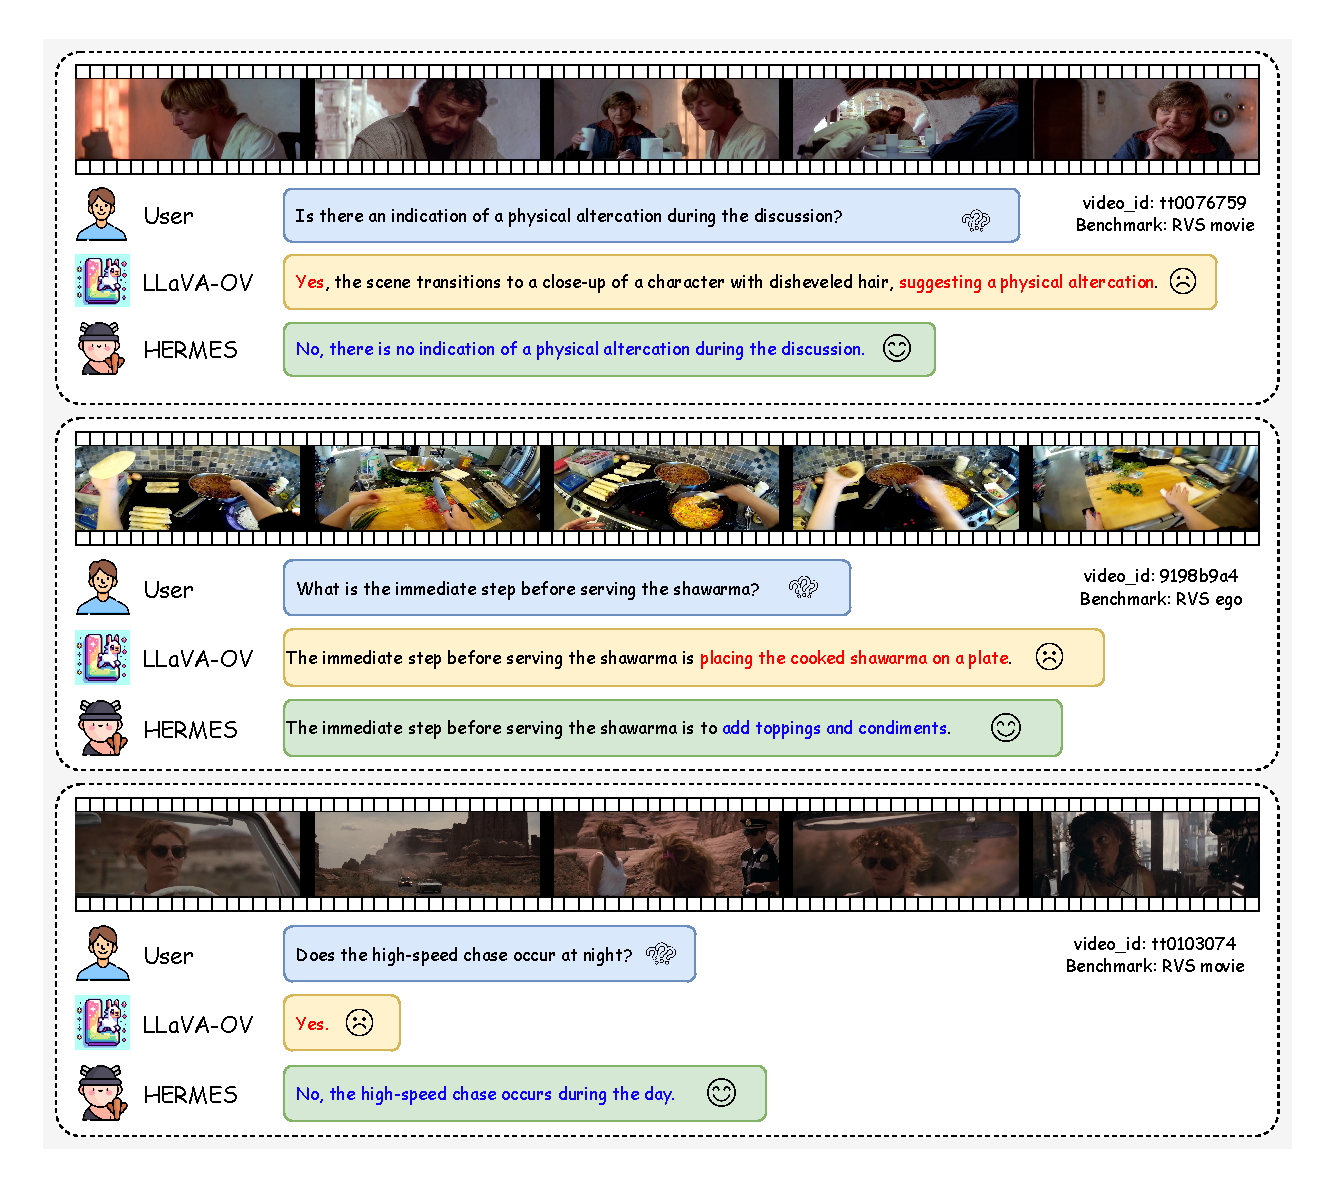
\includegraphics[width=\linewidth]{figures/case_study_temporal.pdf}
  \caption{Cases demonstrating the superior fine-grained temporal understanding capability of \hermes relative to the \llava base model.}
  \label{fig:case_temporal}
\end{figure*}
\begin{figure*}[p]
  \centering
    \includegraphics[width=\linewidth]{figures/case_study_spatial.pdf}
  \caption{Cases demonstrating the superior fine-grained spatial understanding capability of \hermes relative to the \llava base model.}
  \label{fig:case_spatial}
\end{figure*}

\end{document}
